\section{Correctifs apportés à l'inventaire}
    Des correctifs ont été apportés à l'inventaire de manière sporadique. Ça a été particulièrement le cas lorsqu'un gros générateur de déplacement n'avait pas d'estimé de stationnement ou qu'un estimé semblait surestimé. L'approche ici était purement opportuniste et une méthode plus systématique d'estimation pour affecter des estimés à ces propriétés devrait être développé. La figure montre le delta entre l'inventaire réglementaire et un inventaire agrégé où la valeur manuelle est prise en priorité, puis la valeur semi automatique où l'auteur a spécifié les valeurs à utiliser et finalement, l'inventaire réglementaire était choisi pour chaque lot s'il n'y avait pas d'autre estimé. De manière descriptive, les ajustements de la Cité Universitaire sont liés au campus universitaire, au CEGEP et à plusieurs centres commerciaux, l'ajustement dans Lairet est pour le Colisée, et l'ajustement dans le Vieux Limoilou était pour l'hôpital et le CEGEP. L'ajustement dans Saint-Sacrement est pour l'hôpital Jeffrey Hale. Dans le cas de Val-Belair, plusieurs ajustement manuels ont été completés sur des centres commerciaux. Les estimés revus à la baisse sont souvent pour des écoles ou des places d'assemblée où les conversions d'unités étaient problématiques. 
    \begin{figure}[H]
        \centering
        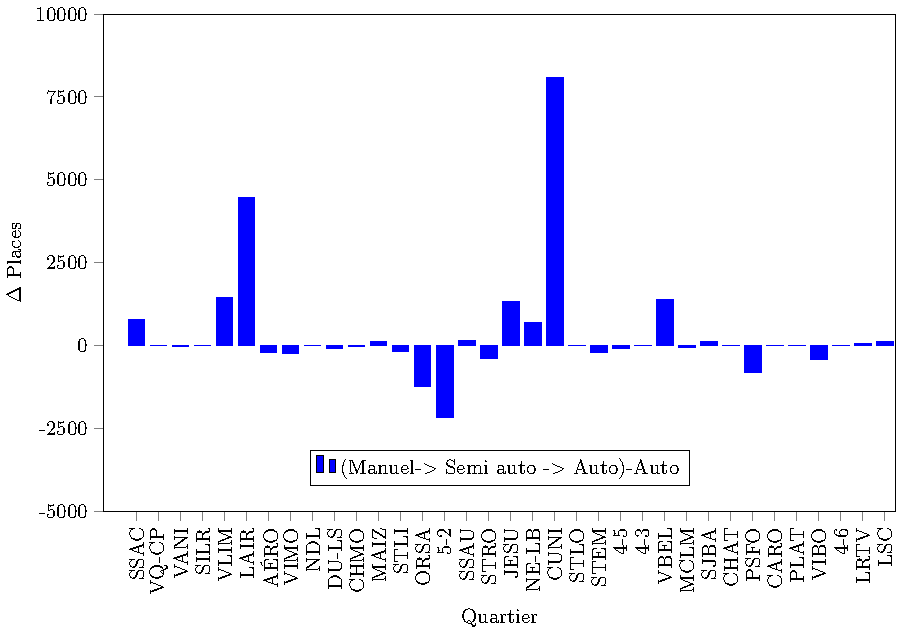
\includegraphics[width=0.8\linewidth]{figures/delta-corrections.pdf}
        \caption{Différence entre l'inventaire corrigé et l'inventaire automatique}
        \label{fig:diff-corrections}
    \end{figure}
\section{Exemples d'analyse}\label{sec:exemples-analyse-resultats}
Cette section montre comment les données pourraient être utilisées pour bonifier la compréhension du stationnement. Les résultats sont purement prospectifs et le fort taux d'absence de données crée des distorsions dans la disponibilité du parc de stationnement. La contribution du stationnement sur rue est complètement évacuée de l'analyse ajoutant un biais supplémentaire. Un important processus d'évaluation des données et de correction est requis pour rendre les constats de cette section valide sur les métriques liées au stationnement. Cela étant dit, la section vise à illustrer un potentiel.\par

La motorisation a été estimée ainsi que les profils d'accumulation véhicule à partir des données de l'enquête OD. Elle est montrée à la figure \ref{fig:motorisation-par-quartier} à titre indicatif pour donner un contexte au reste de l'analyse. 
\begin{figure}[H]
    \centering
    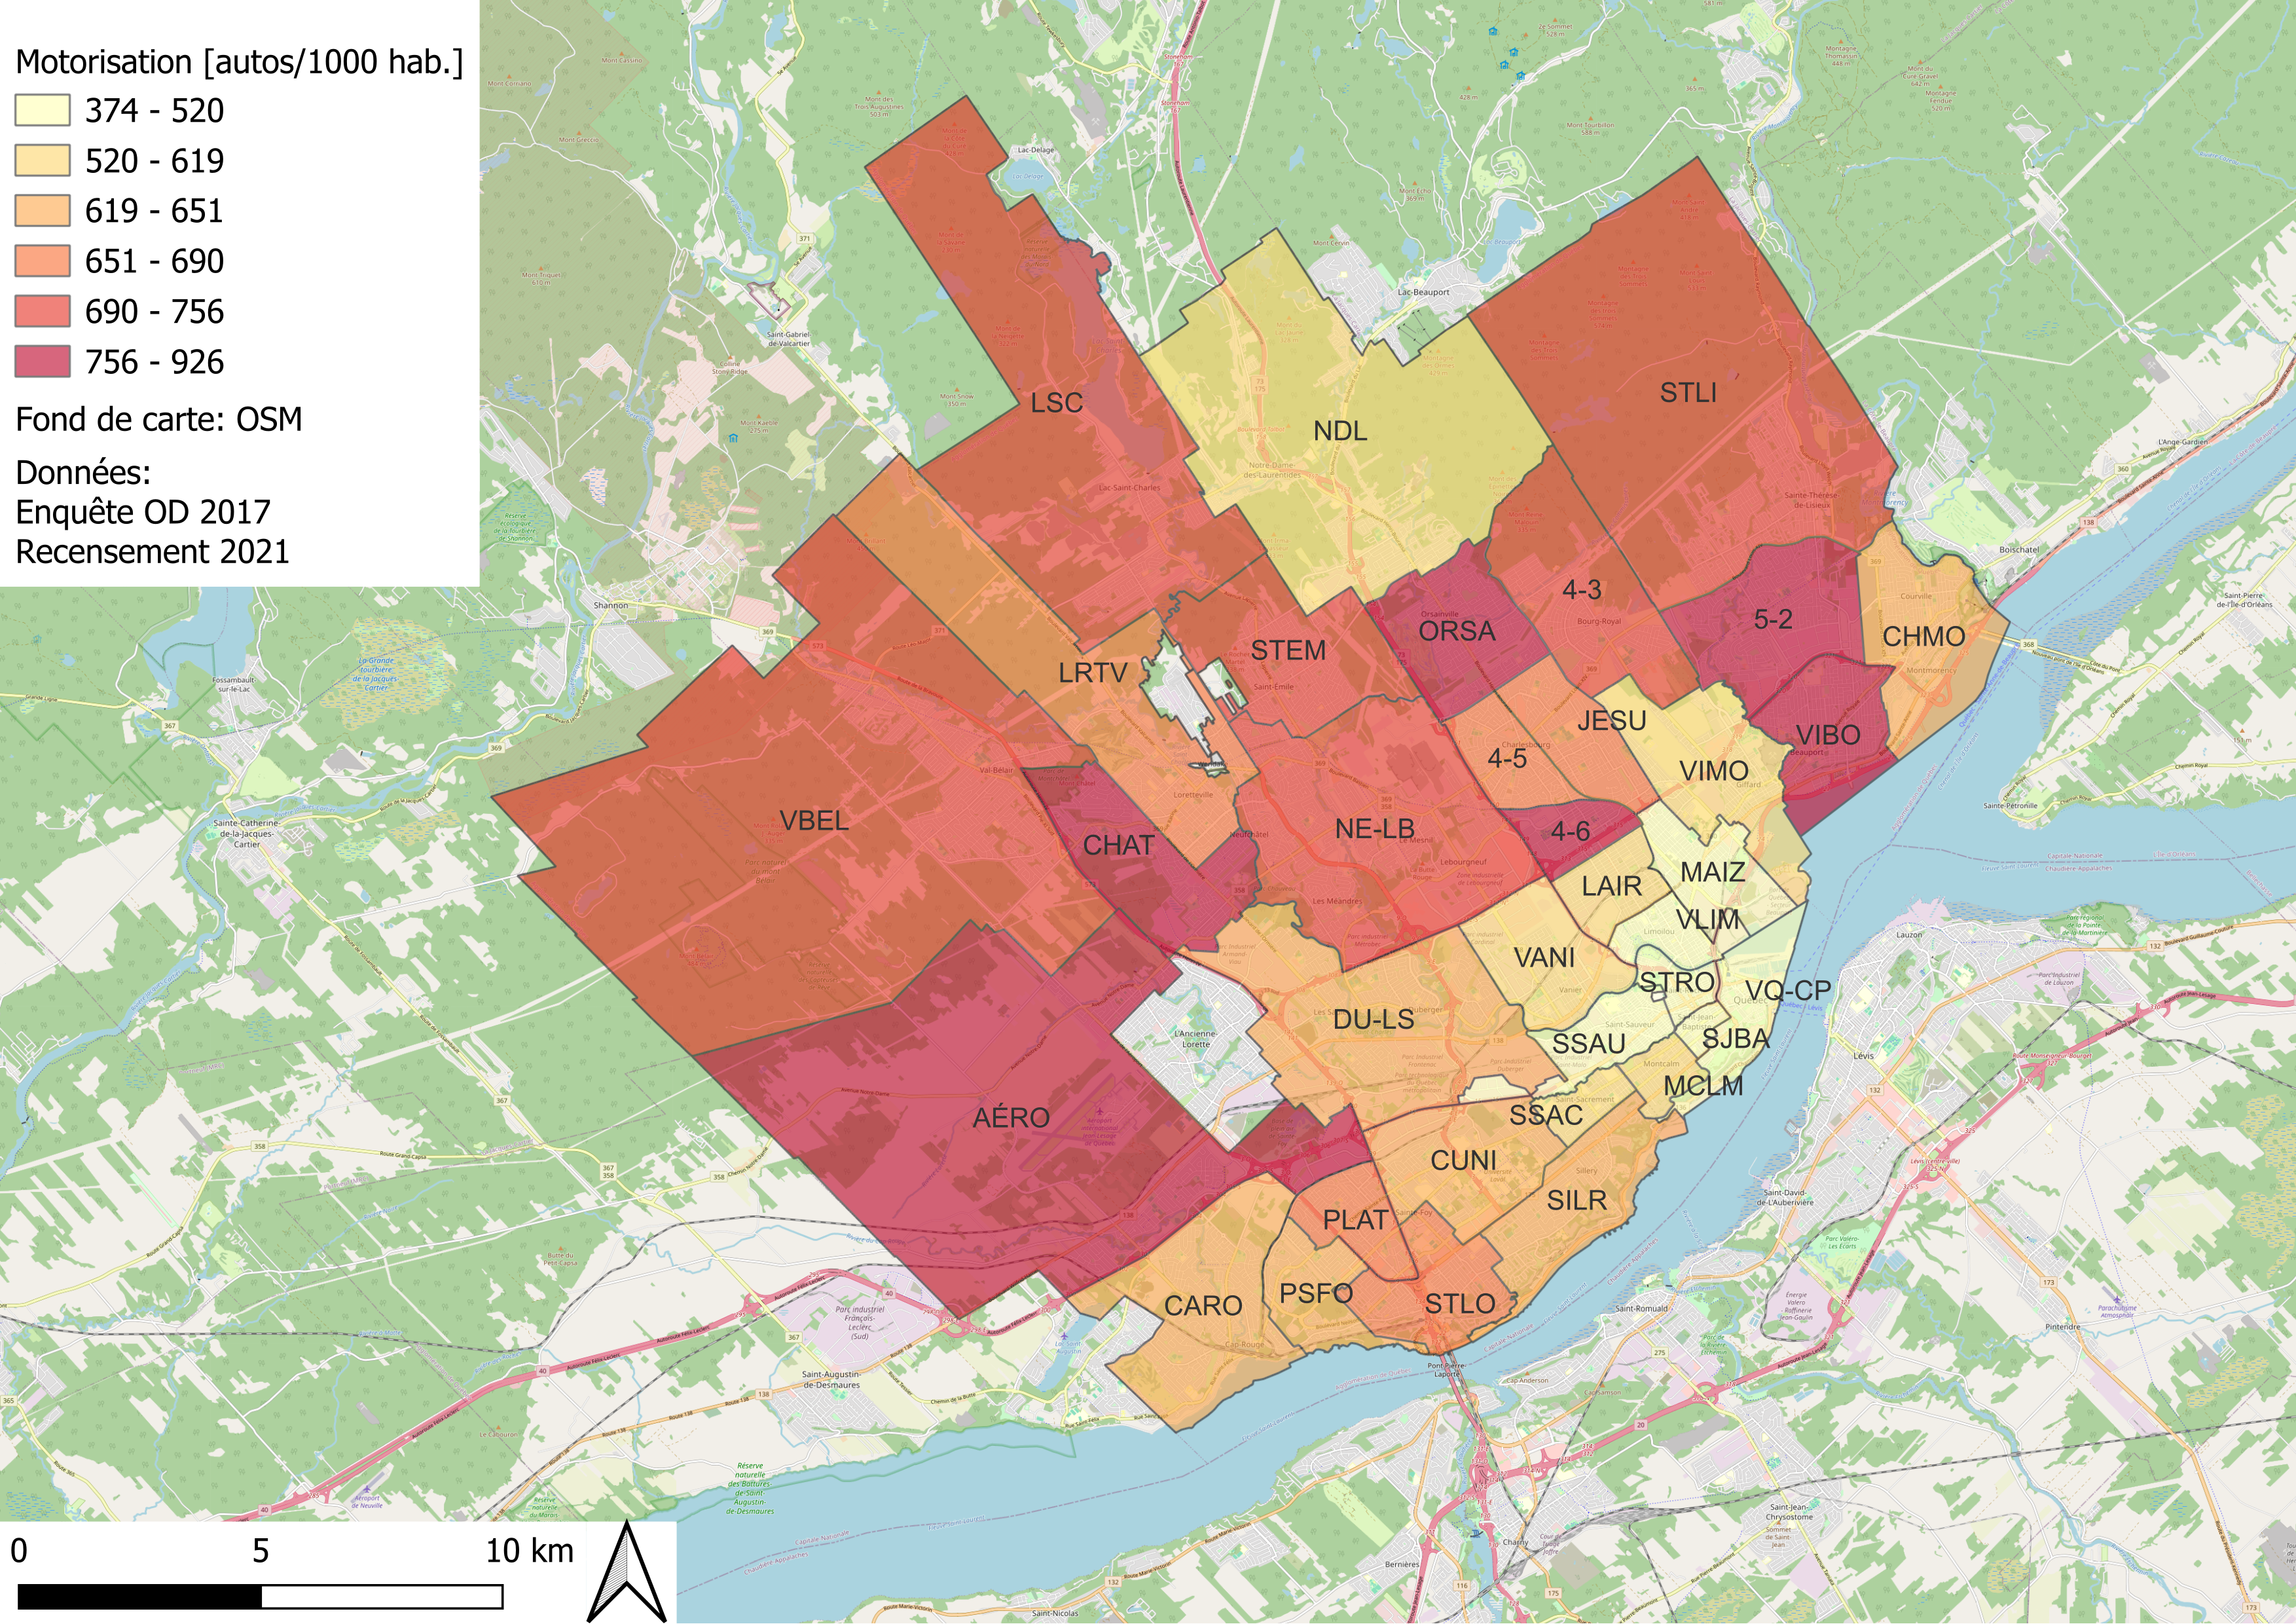
\includegraphics[width=0.8\linewidth]{images/motorisation-par-quartier.png}
    \caption{Motorisation selon les quartiers}
    \label{fig:motorisation-par-quartier}
\end{figure}
On peut ensuite commencer à interroger la mesure dans laquelle le stationnement est saturé. Les figures \ref{fig:places-res-voit-res-hist} et \ref{fig:places-res-voit-res-carte} montrent le nombre de places résidentielles hors-rue par voiture résident. Les résultats montrent qu'il y a plus de places de stationnement par voiture dans les quartier centraux ce qui n'est pas conforme aux attentes puisque les quartiers centraux sont typiquement là où l'on trouve des enjeux de stationnement. L'évaluation du modèle indique que le stationnement résidentiel est sous-estimé dans les lots unifamiliaux qui dominent les quartiers périphériques. L'implémentation d'un portrait juste pour les maisons unifamiliales permettrait de donner un portrait plus juste de l'enjeu.
\begin{figure}[H]
    \centering
    \begin{subfigure}{1\textwidth}
        \centering
        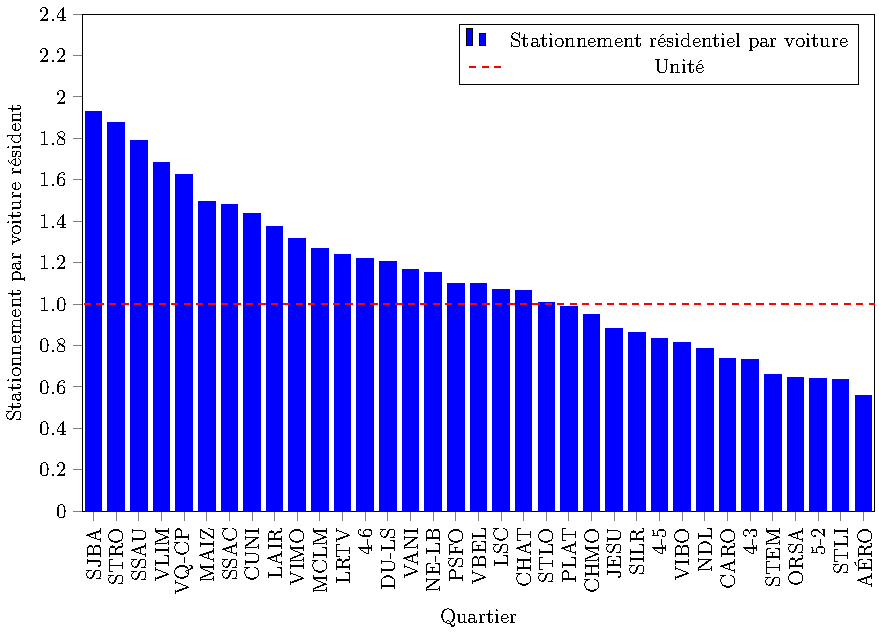
\includegraphics[width=0.75\linewidth]{figures/places-res-par-voit-res.pdf}
        \caption{Histogramme}
        \label{fig:places-res-voit-res-hist}
    \end{subfigure}
    ~
    \begin{subfigure}{1\textwidth}
        \centering
        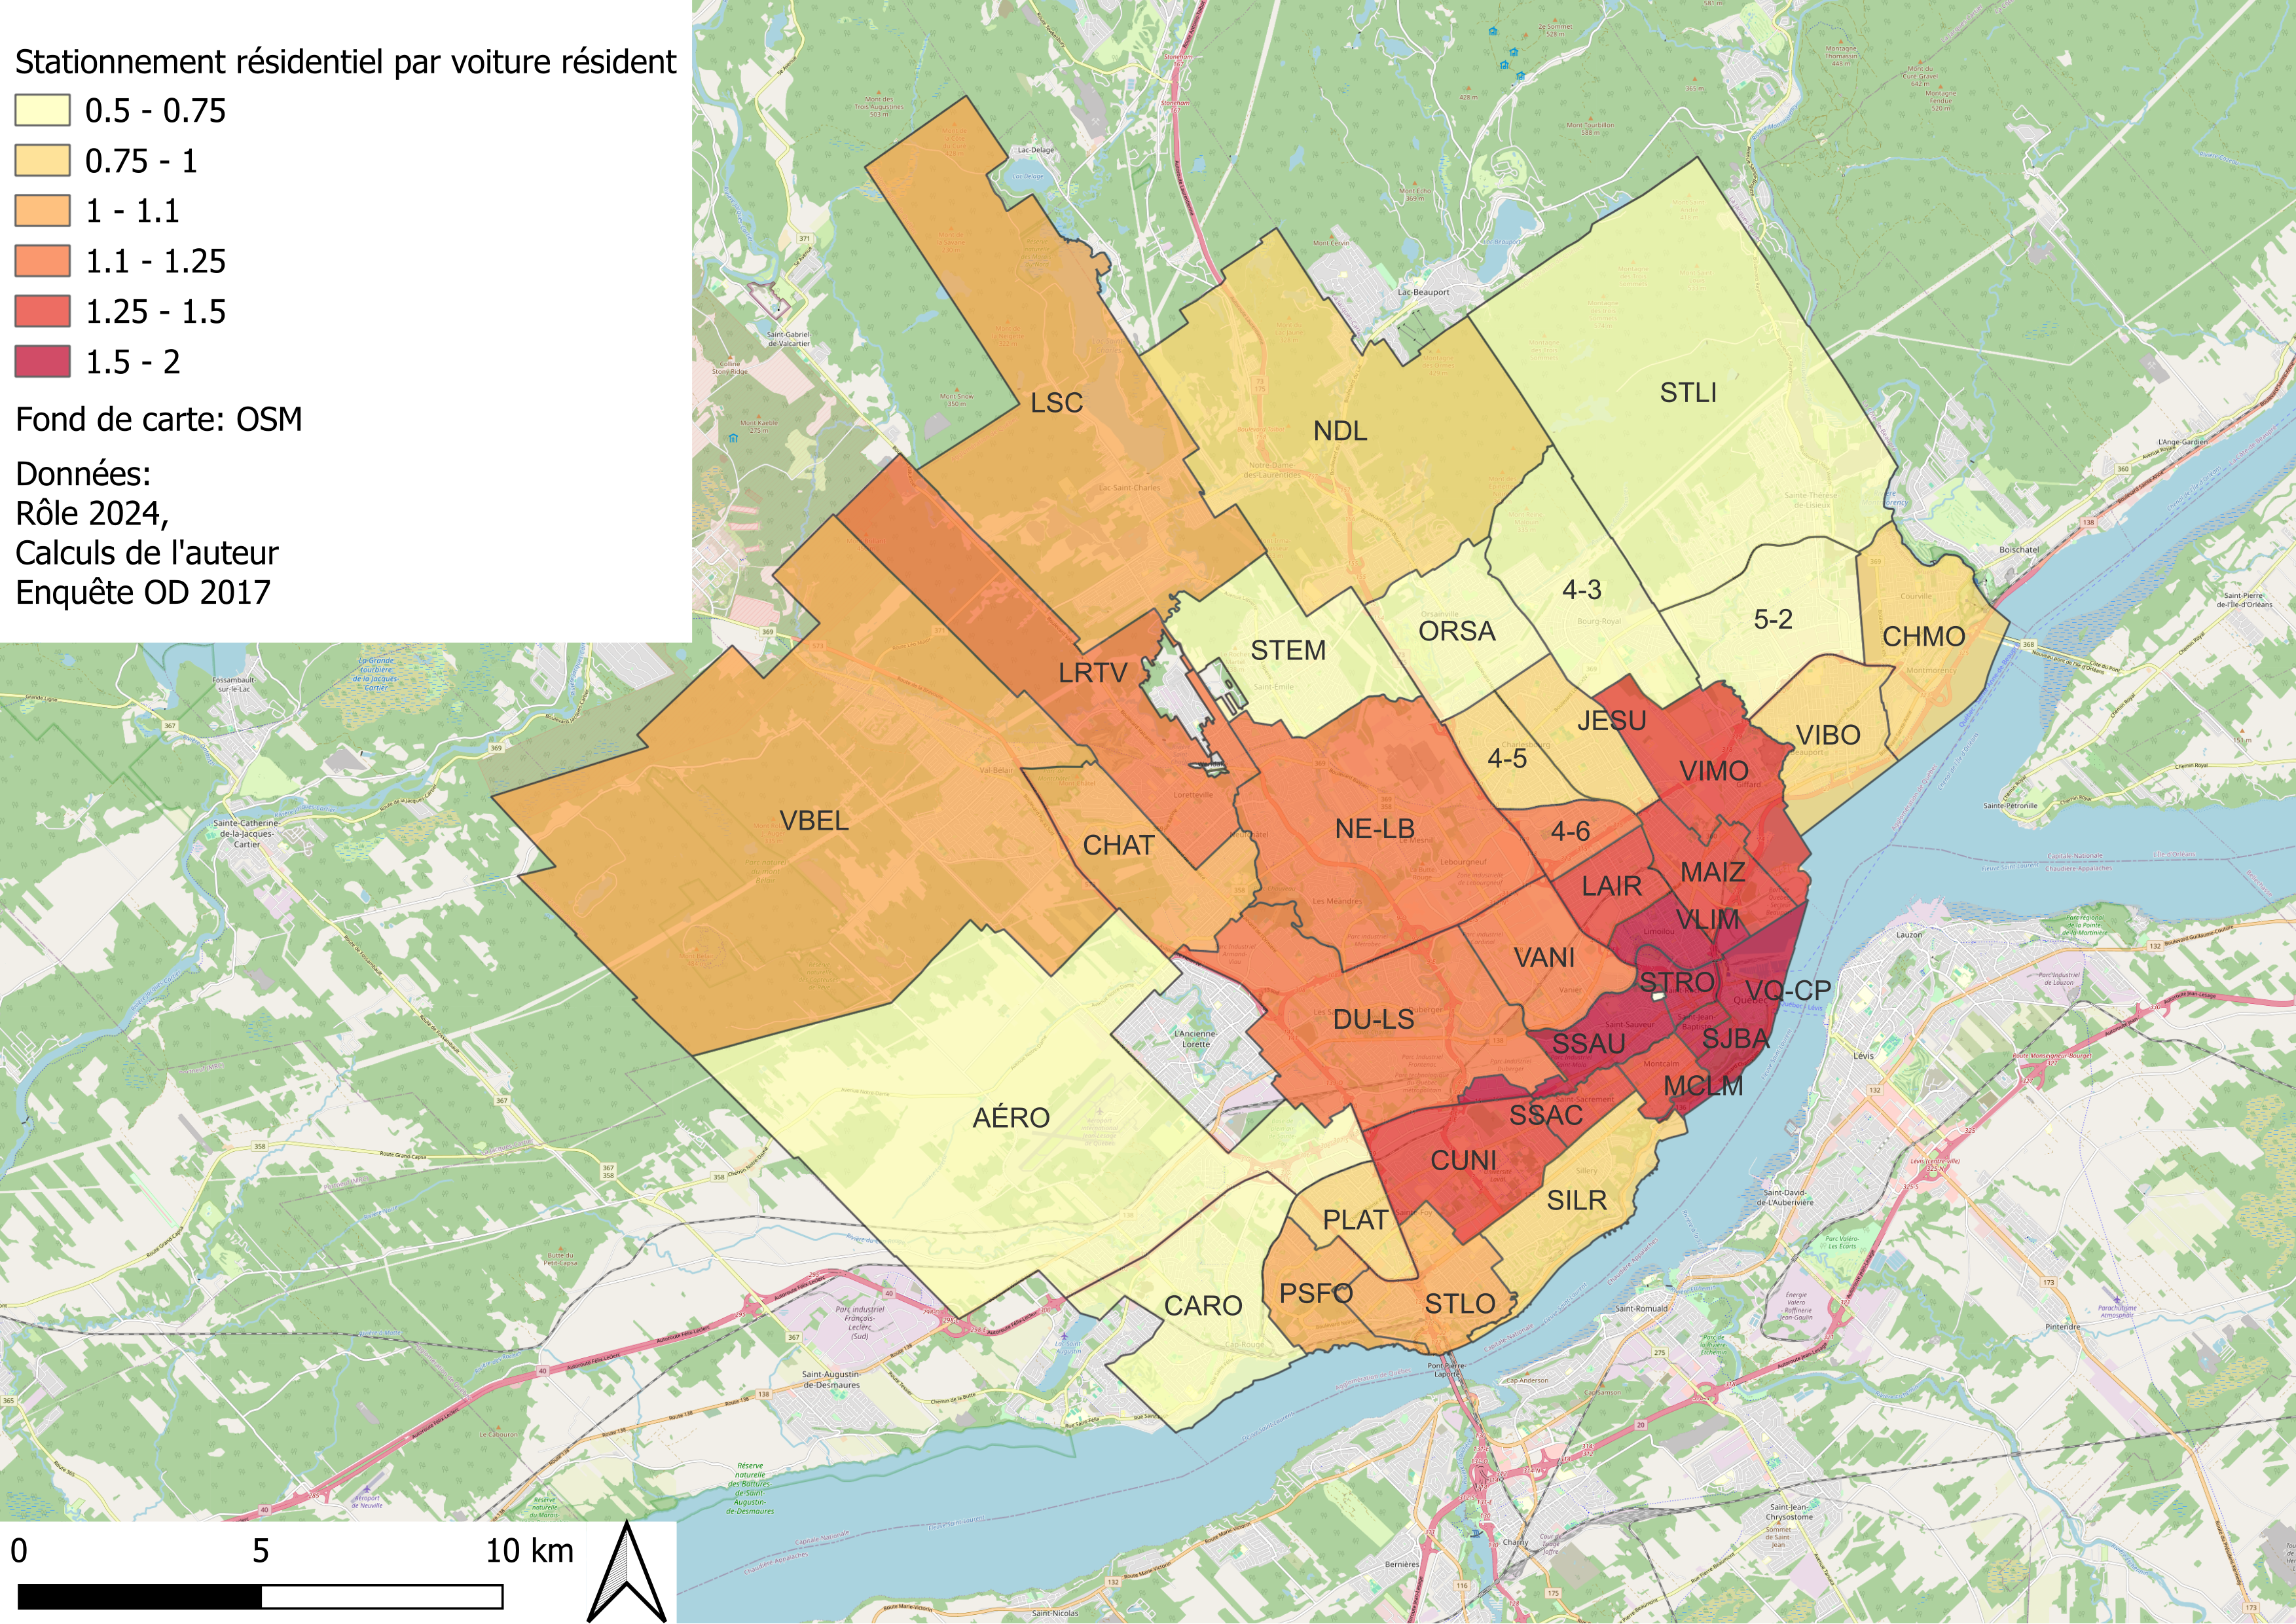
\includegraphics[width=0.75\linewidth]{images/stat-res-par-voit-res.png}
        \caption{Carte}
        \label{fig:places-res-voit-res-carte}
    \end{subfigure}
    \caption{Nombre de places résidentielles par voiture des résidents}
    \label{fig:places-res-voit-res}
\end{figure}
\FloatBarrier

Cependant, même en regardant le nombre de places de stationnement par logement, on constate des tendances contre-intuitives, puisque les quartier centraux paraissent mieux lotis que certains quartiers péri-urbains comme le montre la figure \ref{fig:stationnement-residentiel-par-quartier}. Encore une fois, l'évaluation du modèle montre que ceci est probablement à le biais du modèle pour les propriétés unifamiliales particulièrement lorsqu'on s'éloigne du centre où ce type de logement est plus présent est constitue une plus grande partie du parc de stationnement. 
\begin{figure}[H]
    \centering
    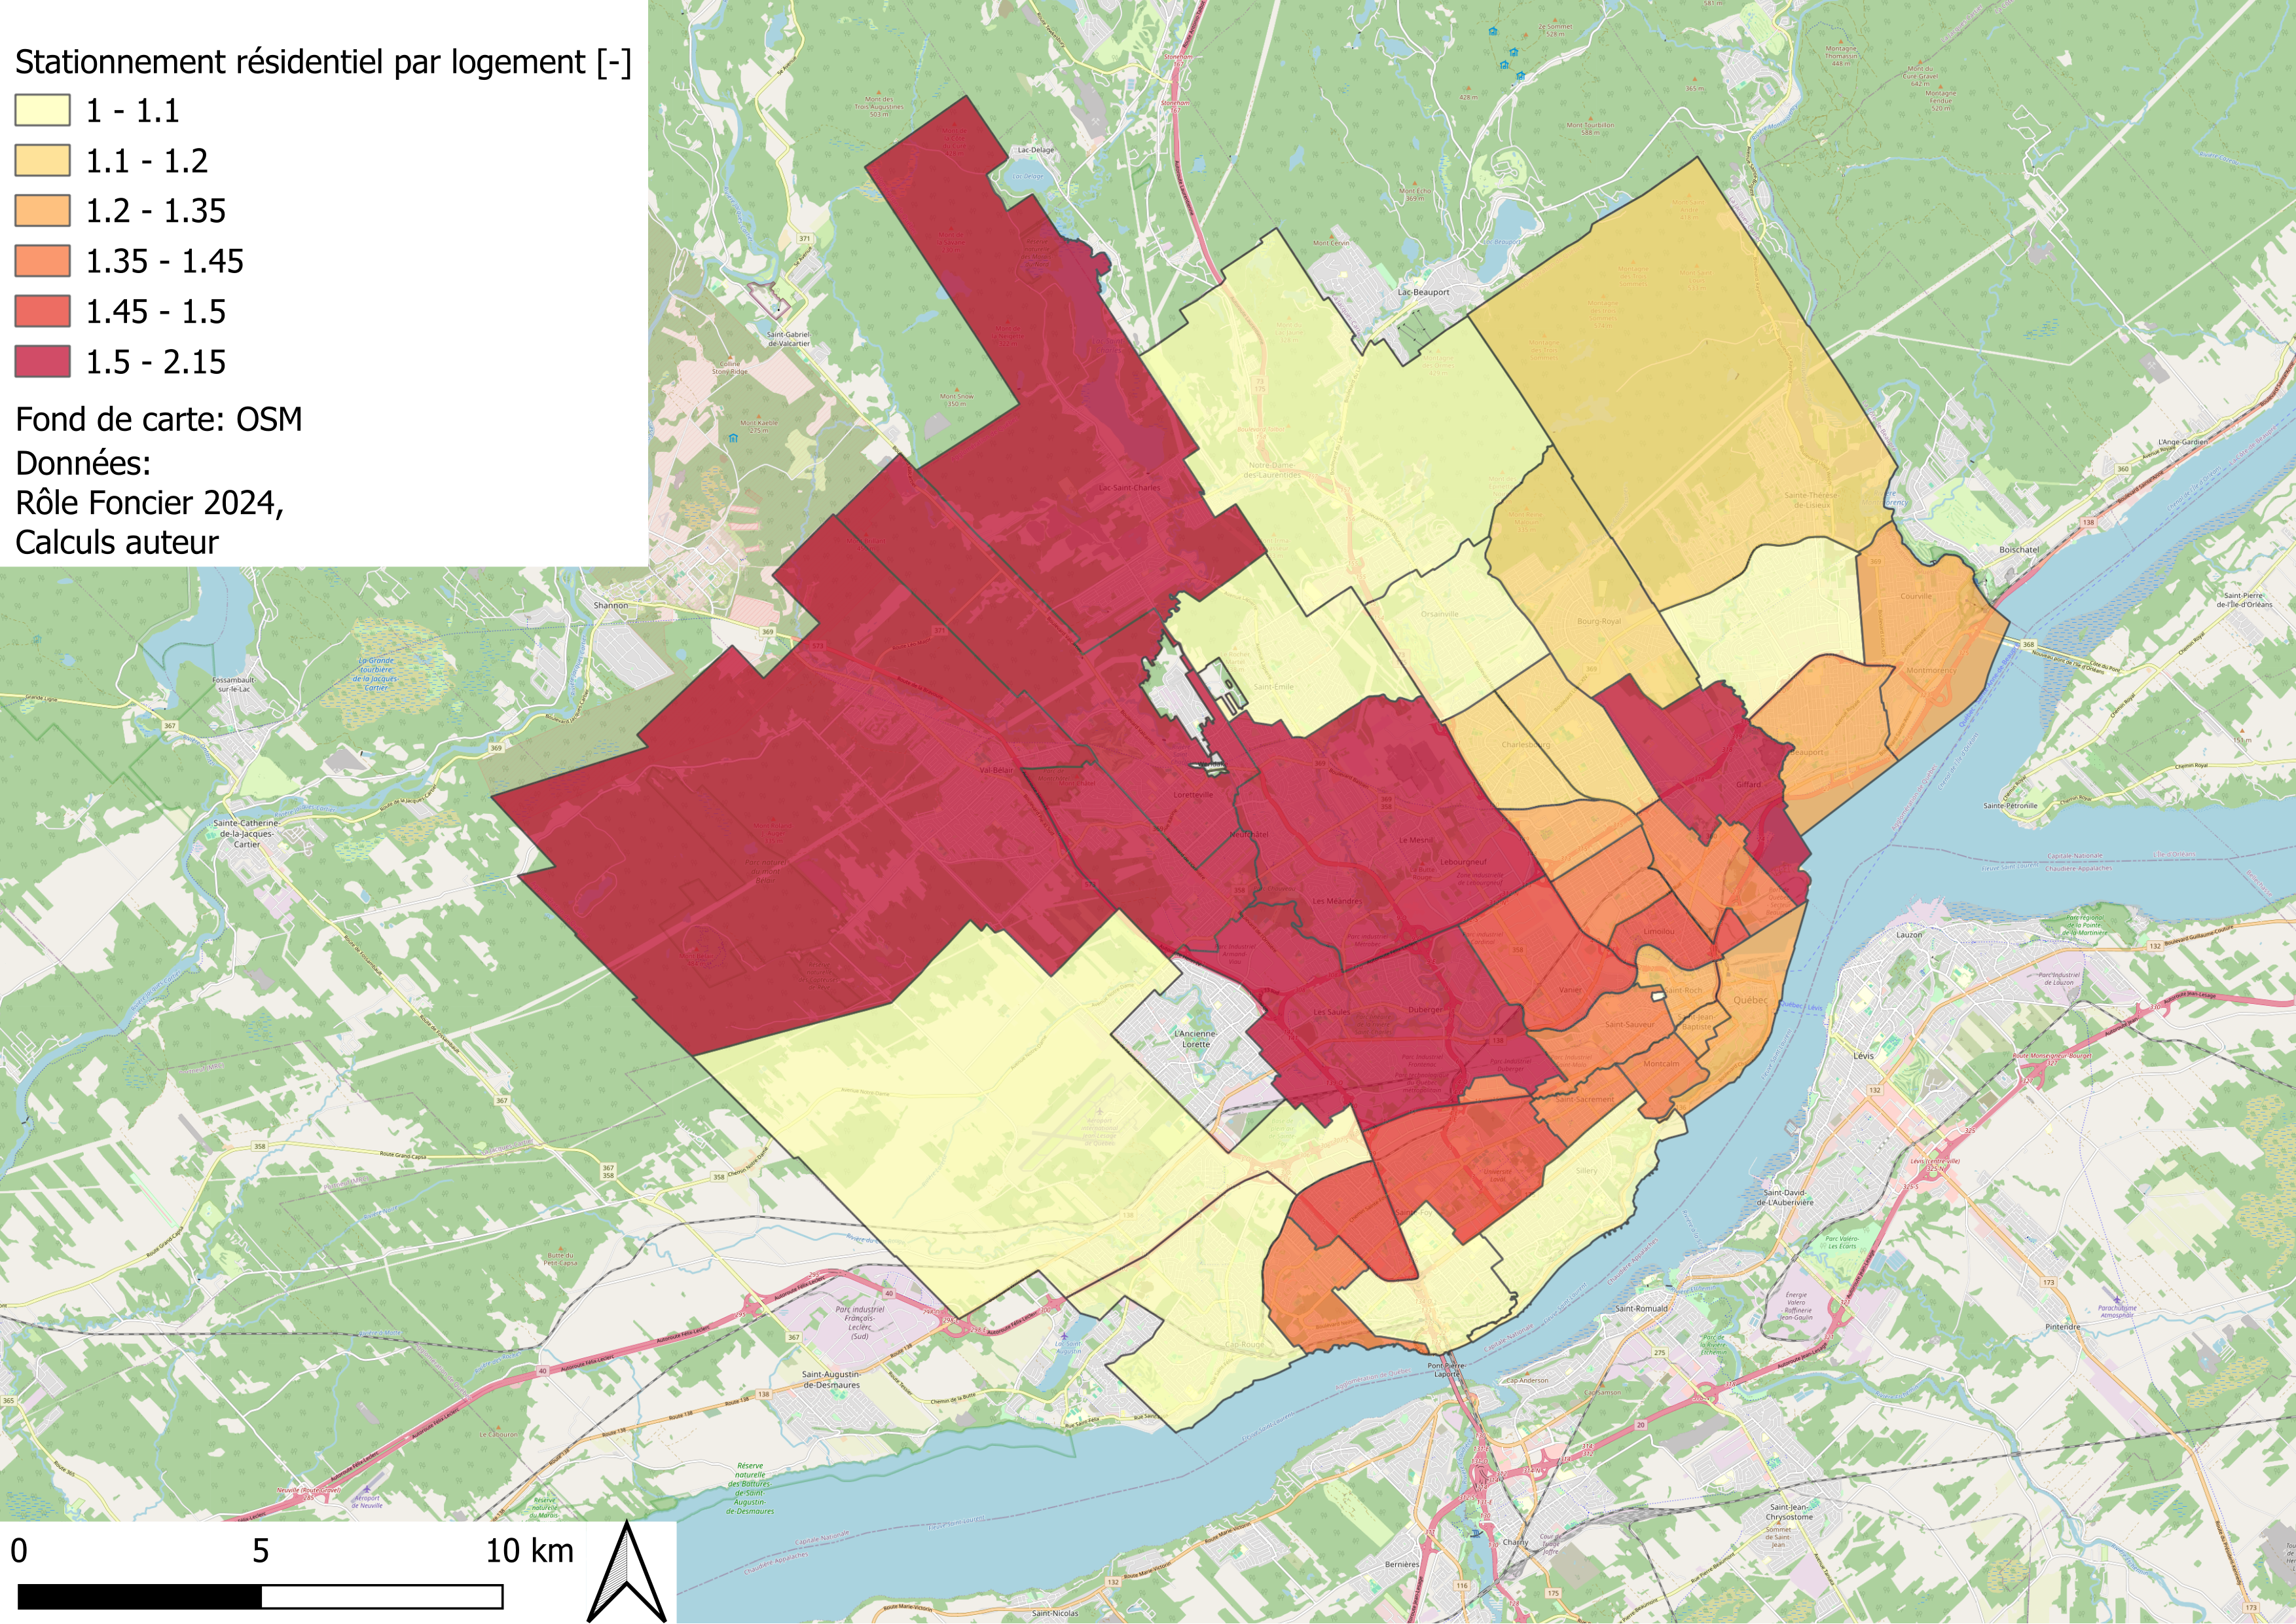
\includegraphics[width=0.8\linewidth]{images/stat-res-par-log.png}
    \caption{Stationnement résidentiel par logement}
    \label{fig:stationnement-residentiel-par-quartier}
\end{figure}
\FloatBarrier
Les profils d'accumulation véhicules peuvent aussi donner une idée de l'utilisation de la capacité. Le parc total de stationnement complet peut être comparé à la population ou la capacité publique (c'est-à-dire autre que résidentielle) peut être comparé aux voitures hors-résidences, donnant potentiellement un meilleur portrait de la compétition aux destinations. La figure \ref{fig:PAV-cite-univ} montre le profile d'accumulation pour la Cité-Universitaire. Les lignes de capacité montrent la capacité réglementaire et une capacité ajustée. La capacité ajustée inclut les stationnement de la place Laurier et de certains stationnement du campus de l'université où les données manquaient.\par
\begin{figure}[H]
    \centering
    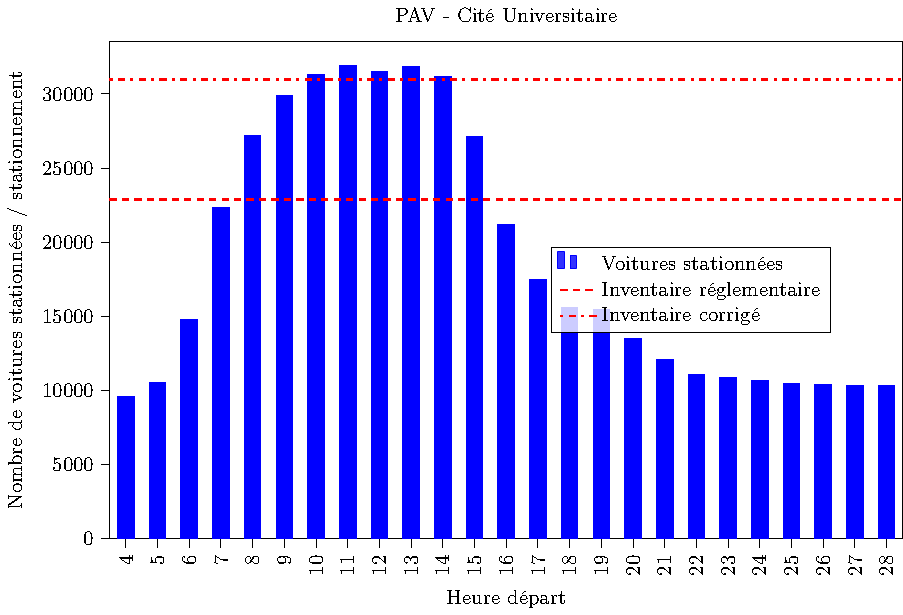
\includegraphics[width=1\linewidth]{figures/basic_PAV_CUNI.pdf}
    \caption{Profile d'accumulation de véhicules de la Cité Universitaire}
    \label{fig:PAV-cite-univ}
\end{figure}


Ce même exercice peut aussi être fait en isolant les voitures stationnées à la résidence ou dans un stationnement public. Les figure \ref{fig:pav-resi-cuni} et \ref{fig:pav-public-cuni} montrent l'accumulation de véhicules à la résidence contre la capacité résidentielle, et la même pour chose pour les places publiquement accessibles(autres que résidentielles). 
\begin{figure}[H]
    \centering
    \begin{subfigure}{1\textwidth}
        \centering
        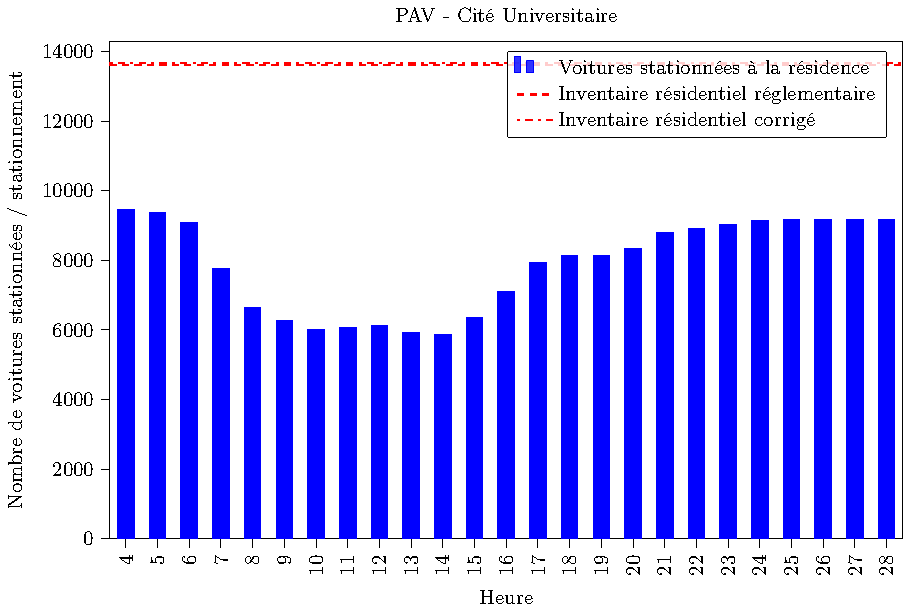
\includegraphics[width=0.8\linewidth]{figures/residential_PAV_CUNI.pdf}
        \caption{Résidentiel}\label{fig:pav-resi-cuni}
    \end{subfigure}
    \begin{subfigure}{1\textwidth}
        \centering
        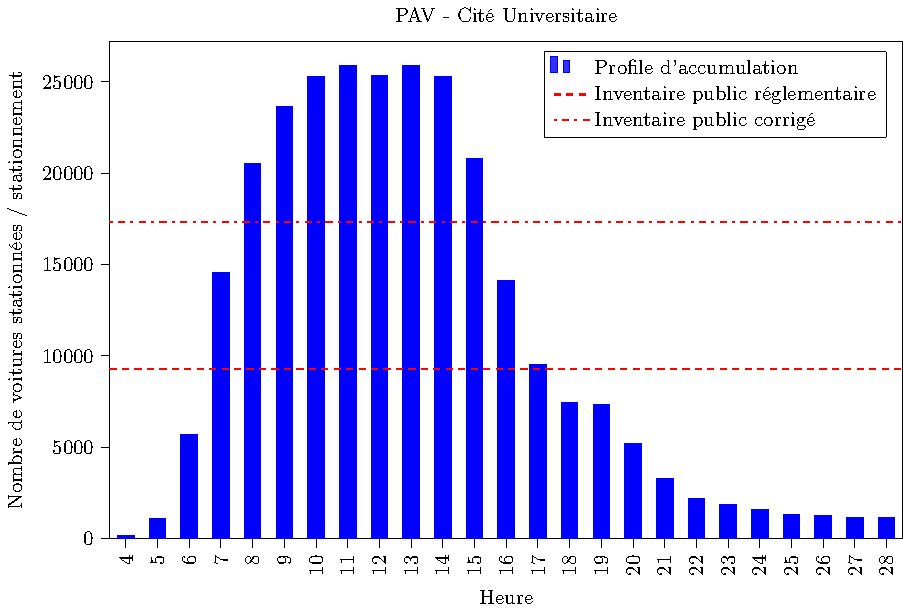
\includegraphics[width=0.8\linewidth]{figures/pub_PAV_CUNI.pdf}
        \caption{Destination}\label{fig:pav-public-cuni}
    \end{subfigure}
    \caption{Profiles d'accumulation de véhicules par clientèle}
    \label{fig:pav-by-clientele}
\end{figure}\clearpage
On constate qu'il y a un grand manque à gagner dans les places de stationnement public. Des enjeux demeurent quant à la précision de l'inventaire et le fait de ne pas inclure le stationnement sur rue limite les possibilités d'interprétation.\par
La création de profils d'accumulation de personnes et de permis peuvent aussi être complétés pour la même zone et permet d'inférer la consommation d'espace supplémentaire si chaque personne venait en automobile. La différentiation entre personnes et permis est mise en place pour comprendre quelles sont les personnes qui peuvent conduire qui ne viennent pas dans le quartier en voiture. Les figures \ref{fig:PAPERS-cuni} et \ref{fig:PAPERM-cuni} montrent comment la situation comment il y a beaucoup plus de personnes, détenteurs de permis ou non qui rentrent sur le territoire de la Cité-Universitaire. \par
La dynamique montrée pour la Cité-Universitaire n'est cependant pas la même que pour des quartiers plus excentrés qui sont plus des communautés dortoirs. La figure \ref{fig:pav-basic-orsa} montre le profile d'accumulation de base pour le quartier d'Orsainville qui se vide pendant la journée et où le stationnement résidentiel constitue 65\% de l'inventaire réglementaire (7882 places). Encore une fois, on constate que le stationnement prédit ne permet pas d'entreposer l'ensemble de la demande, menant à des questions sur la disponibilité du stationnement sur-rue et la fiabilité de l'inventaire. 
\begin{figure}[H]
    \centering
    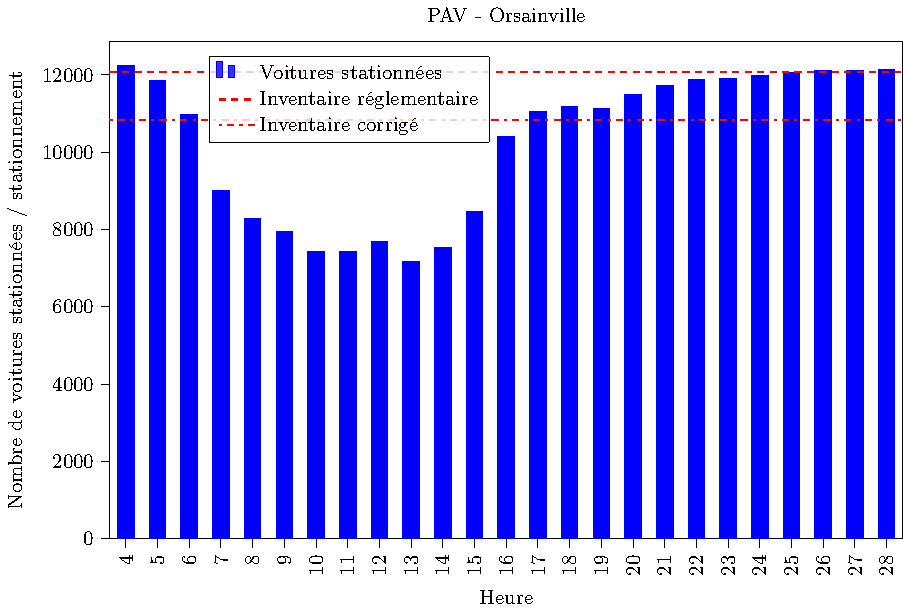
\includegraphics[width=0.75\linewidth]{figures/basic_PAV_ORSA.pdf}
    \caption{Profile d'accumulation d'Orsainville}
    \label{fig:pav-basic-orsa}
\end{figure}
\begin{figure}[H]
    \centering
    \begin{subfigure}{1\textwidth}
        \centering
        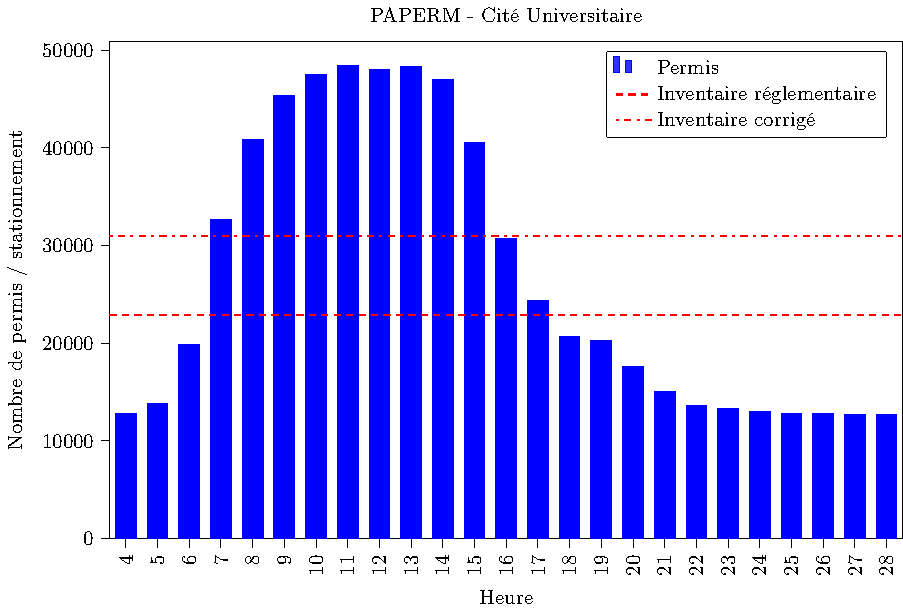
\includegraphics[width=0.8\linewidth]{figures/PAPERM_CUNI.pdf}
        \caption{Permis}\label{fig:PAPERM-cuni}
    \end{subfigure}
    \begin{subfigure}{1\textwidth}
        \centering
        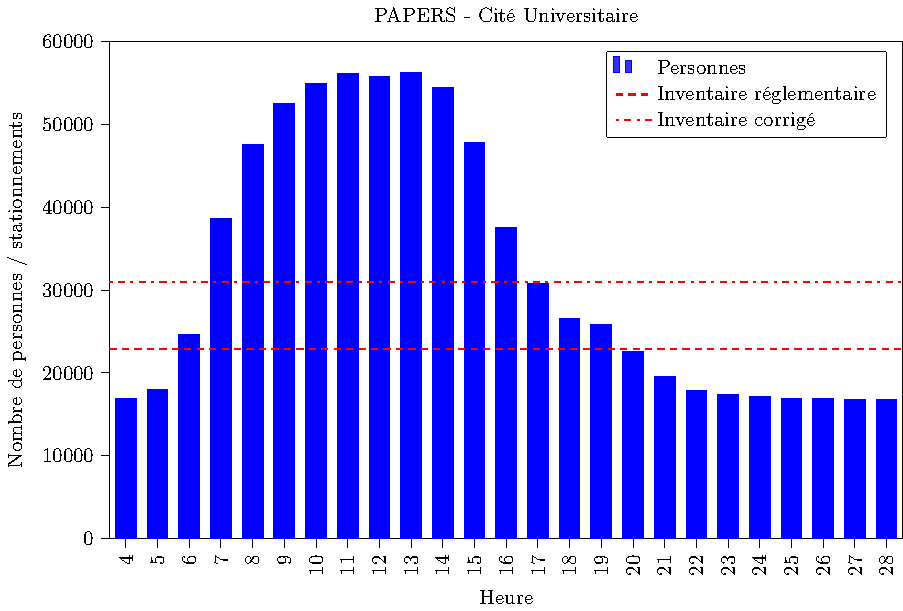
\includegraphics[width=0.8\linewidth]{figures/PAPERS_CUNI.pdf}
        \caption{Personnes}\label{fig:PAPERS-cuni}
    \end{subfigure}
    \caption{Profiles d'accumulation de personnes et permis pour la Cité Universitaire}
    \label{fig:pap-cuni}
\end{figure}\clearpage

La figure \ref{fig:reg-logement-vigueur-1997} montre un graphique créé dans Python en faisant l'appel d'\ac{API} pour obtenir les données. On constate une forte variabilité entre les différent juridictions. 
\begin{figure}[H]
    \centering
    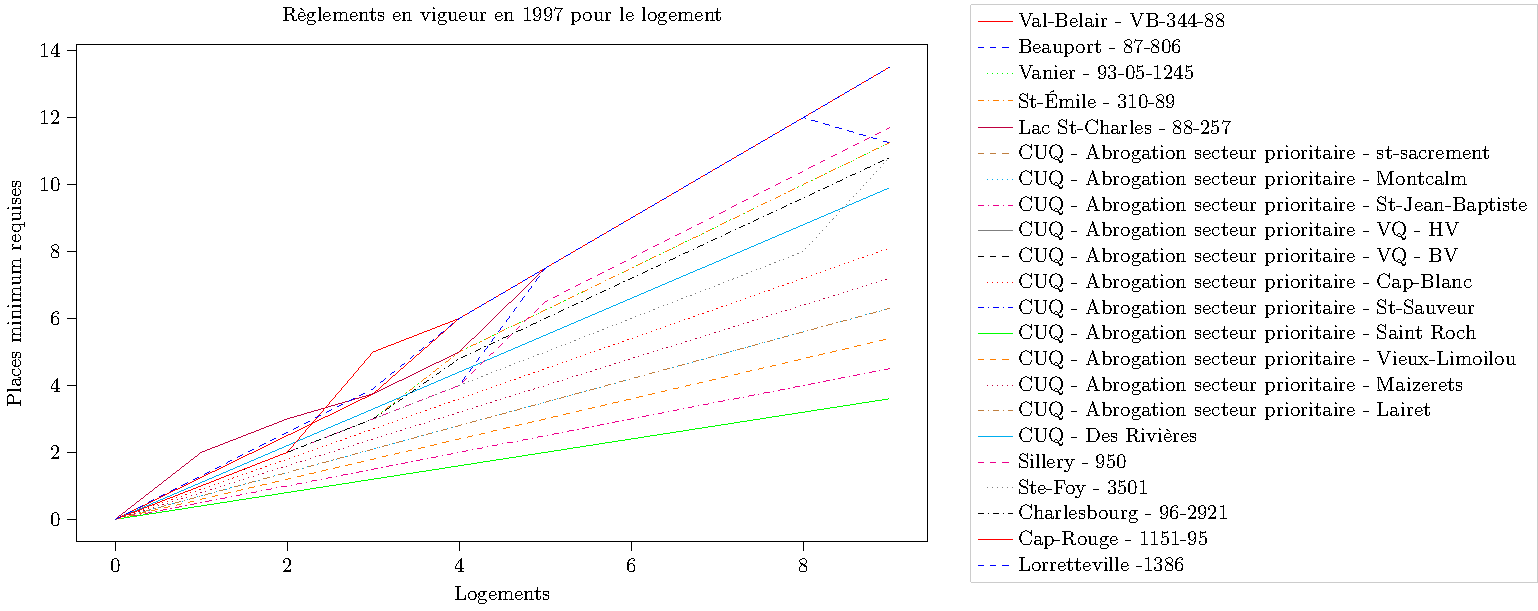
\includegraphics[width=0.8\linewidth]{figures/comparaisonReglement1997Resident.pdf}
    \caption{Comparaison des règlements de stationnement en vigueur en 1997 pour le logement}
    \label{fig:reg-logement-vigueur-1997}
\end{figure}

L'analyse de variabilité peut servir à comprendre comment les politiques de stationnement auraient pu affecter la production de stationnement. Ici, tous les ensembles de règlements sont appliqués à toutes les entrées du rôle et seulement le total est comparé. L'approche permet cependant de montrer à quel point les minimums peuvent avoir de l'influence s'ils sont contraignants pour les développeurs immobiliers comme l'indique la littérature \parencite{cutter_parking_2012,li_parking_2014,smith_low-rise_1964}
\begin{figure}[H]
    \centering
    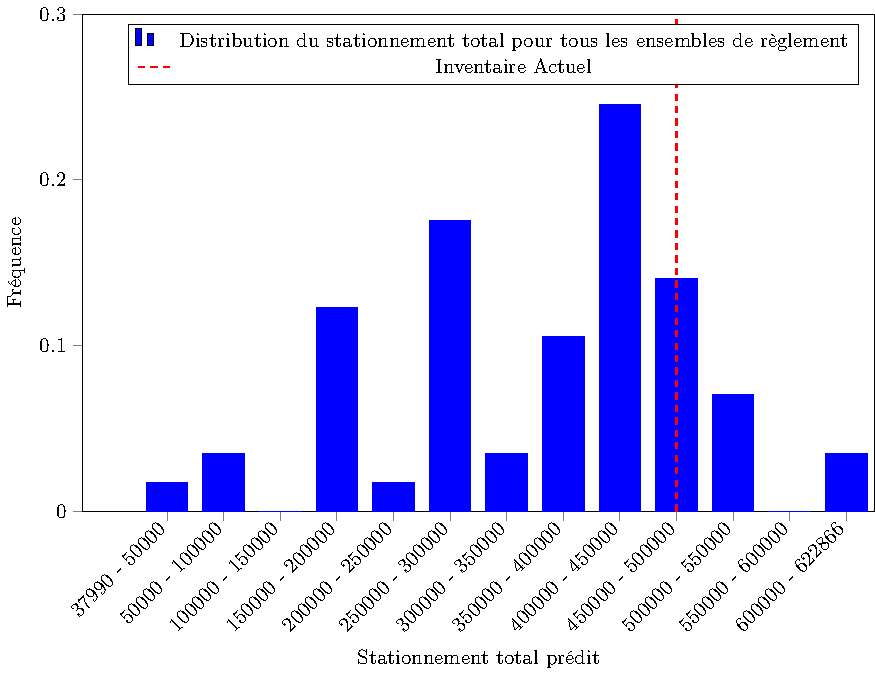
\includegraphics[width=0.6\linewidth]{figures/ana-var-tot.pdf}
    \caption{Exemple d'analyse de variation utilisant tous les ensembles de règlements}
    \label{fig:ana-var-example}
\end{figure}
Les prédiction peuvent aussi être utilisés pour pour estimer le pourcentage du territoire dédié au stationnement. Les quartiers voient une part plus grande de leur territoire dédié au stationnement. 
\begin{figure}[H]
    \centering
    \begin{subfigure}{1\textwidth}
        \centering
        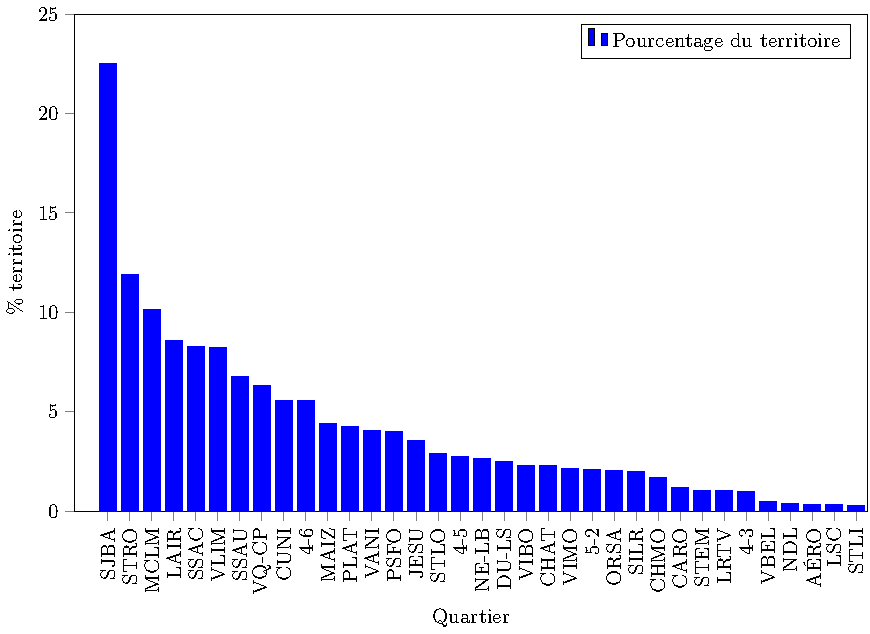
\includegraphics[width=0.675\linewidth]{figures/pourcent_territoire.pdf}
        \caption{Barres}
    \end{subfigure}
    \begin{subfigure}{1\textwidth}
        \centering
        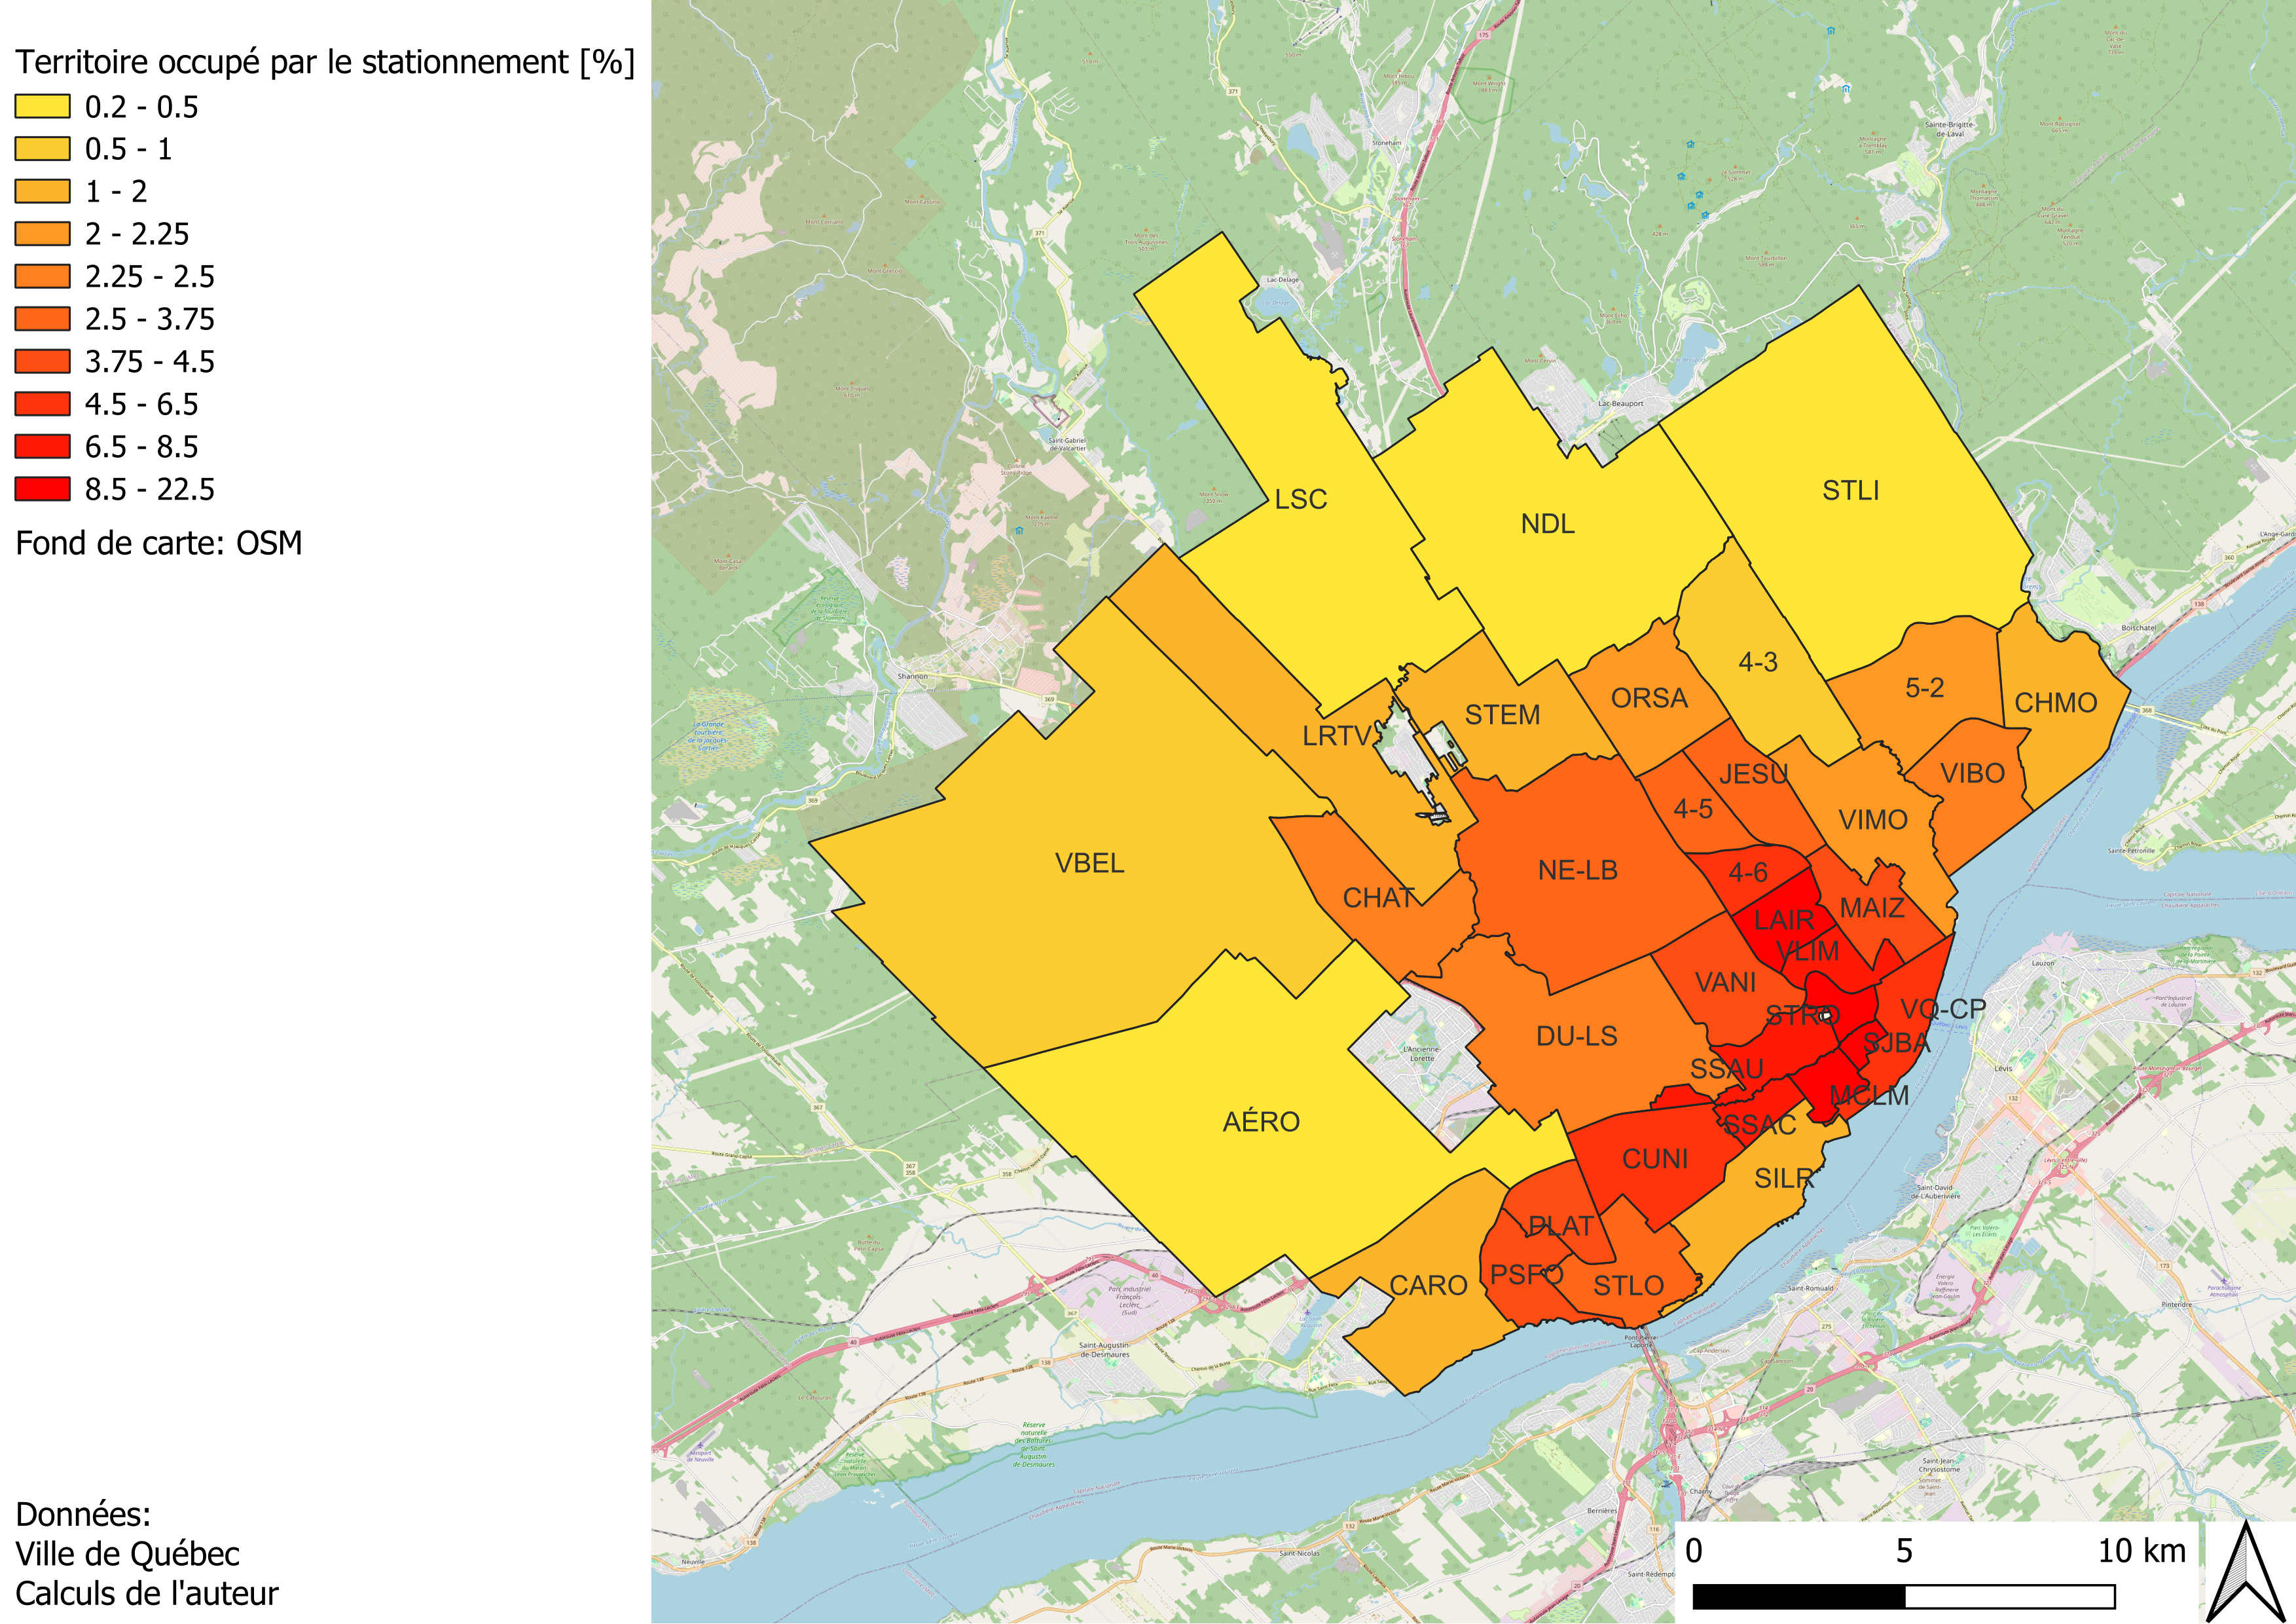
\includegraphics[width=0.675\linewidth]{images/perc-terr-stat.png}
        \caption{Carte}
    \end{subfigure}
    \caption{Pourcentage du territoire dédié au stationnement par quartier}\label{fig:perc-terr-occ-stat}
\end{figure}
Plusieurs facteurs contribuent à ce résultat, l'utilisation du sol variant selon les secteurs, l'absence de compensation pour le fait qu'un partie du stationnement est souterraine ou en étages dans les quartier centraux et la variation du taux de données absentes selon l'utilsation du sol et le quartier.\par

On peut aussi déduire des taux d'occupation théoriques des quartiers à partir des profils d'accumulation de véhicules. En prenant la valeur maximale du profile d'accumulation et en la comparant au parc de stationnement prédit, il est possible de dresser un portrait de l'utilisation de la capacité. Ce portrait peut être dressé par catégorie. On peut déduire un taux d'occupation total maximal ou le différencier pour le parc public (usages autres que résidentiel) ou pour le parc résidentiel. Évidemment, les maximums d'occupation n'ont pas nécessairement lieu en même temps. La figure \ref{fig:occupancy-rate-total} montre le taux d'occupation pour le parc total. Les valeurs excèdent très largement 100\%
\begin{figure}[H]
    \centering
    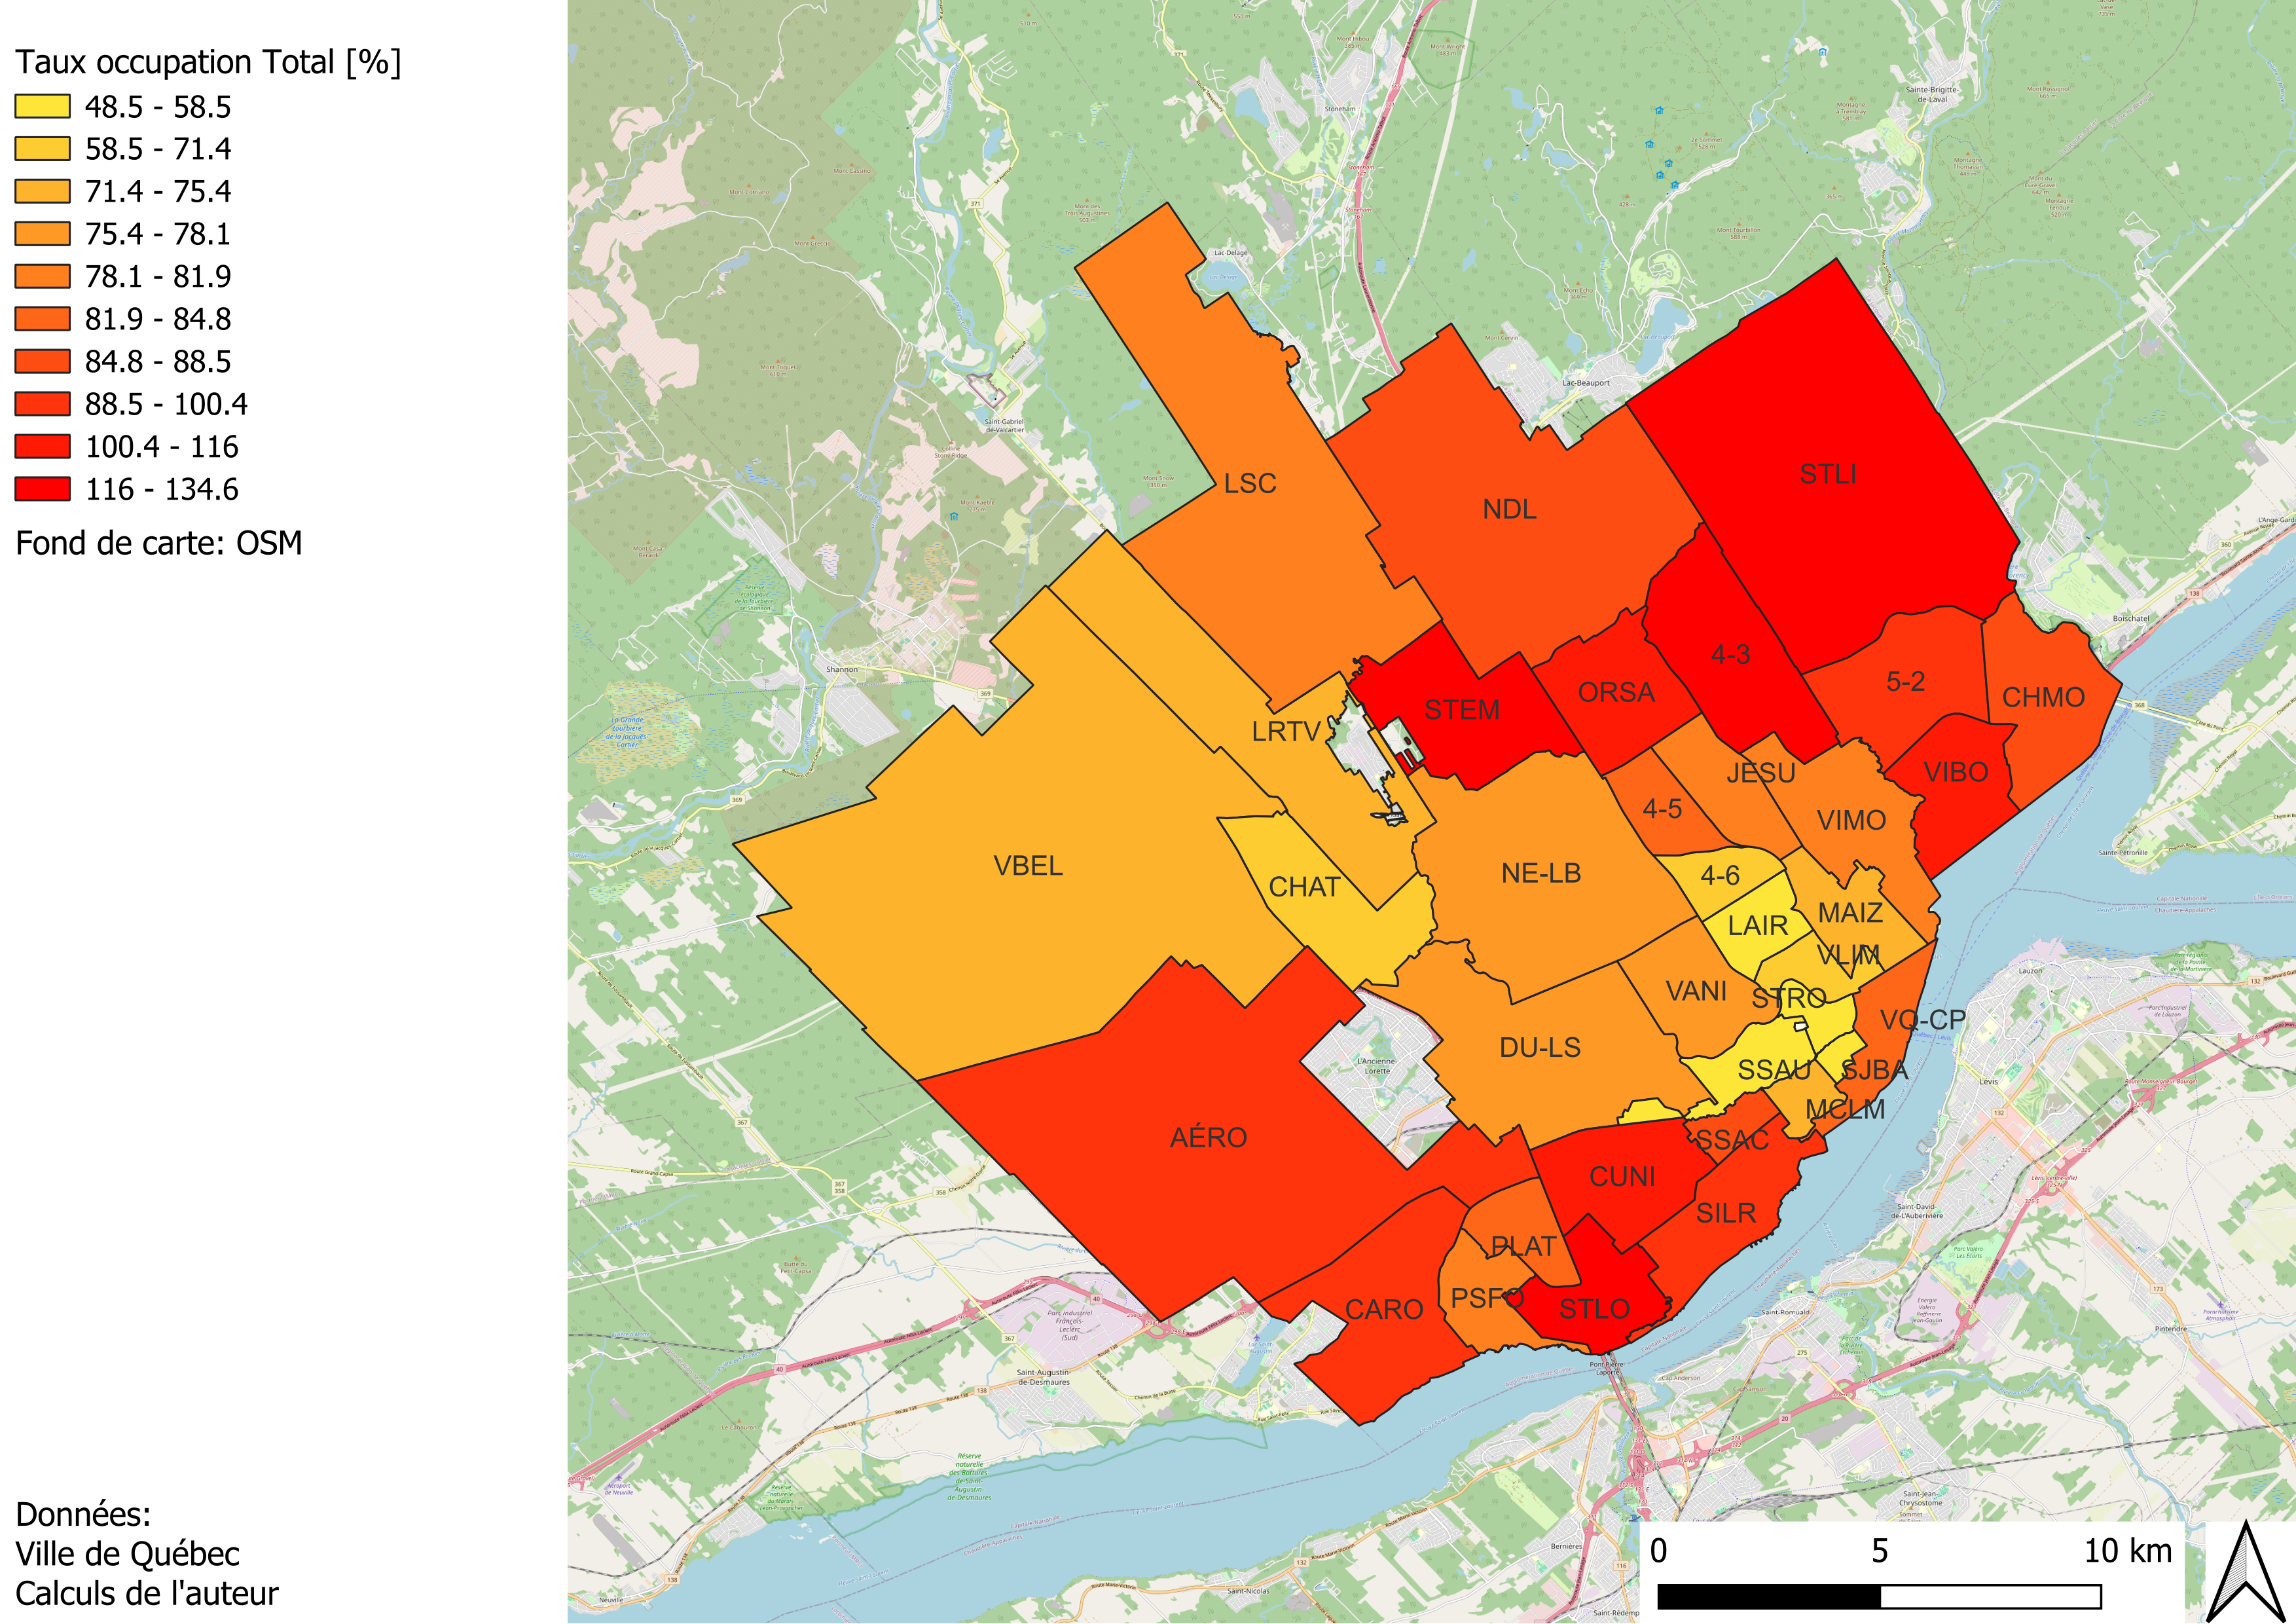
\includegraphics[width=0.8\linewidth]{images/taux-occup-total.png}
    \caption{Taux d'occupation total maximal prédit }
    \label{fig:occupancy-rate-total}
\end{figure}\clearpage
Une carte similaire peut être créée pour le parc de stationnement public 
\begin{figure}[H]
    \centering
    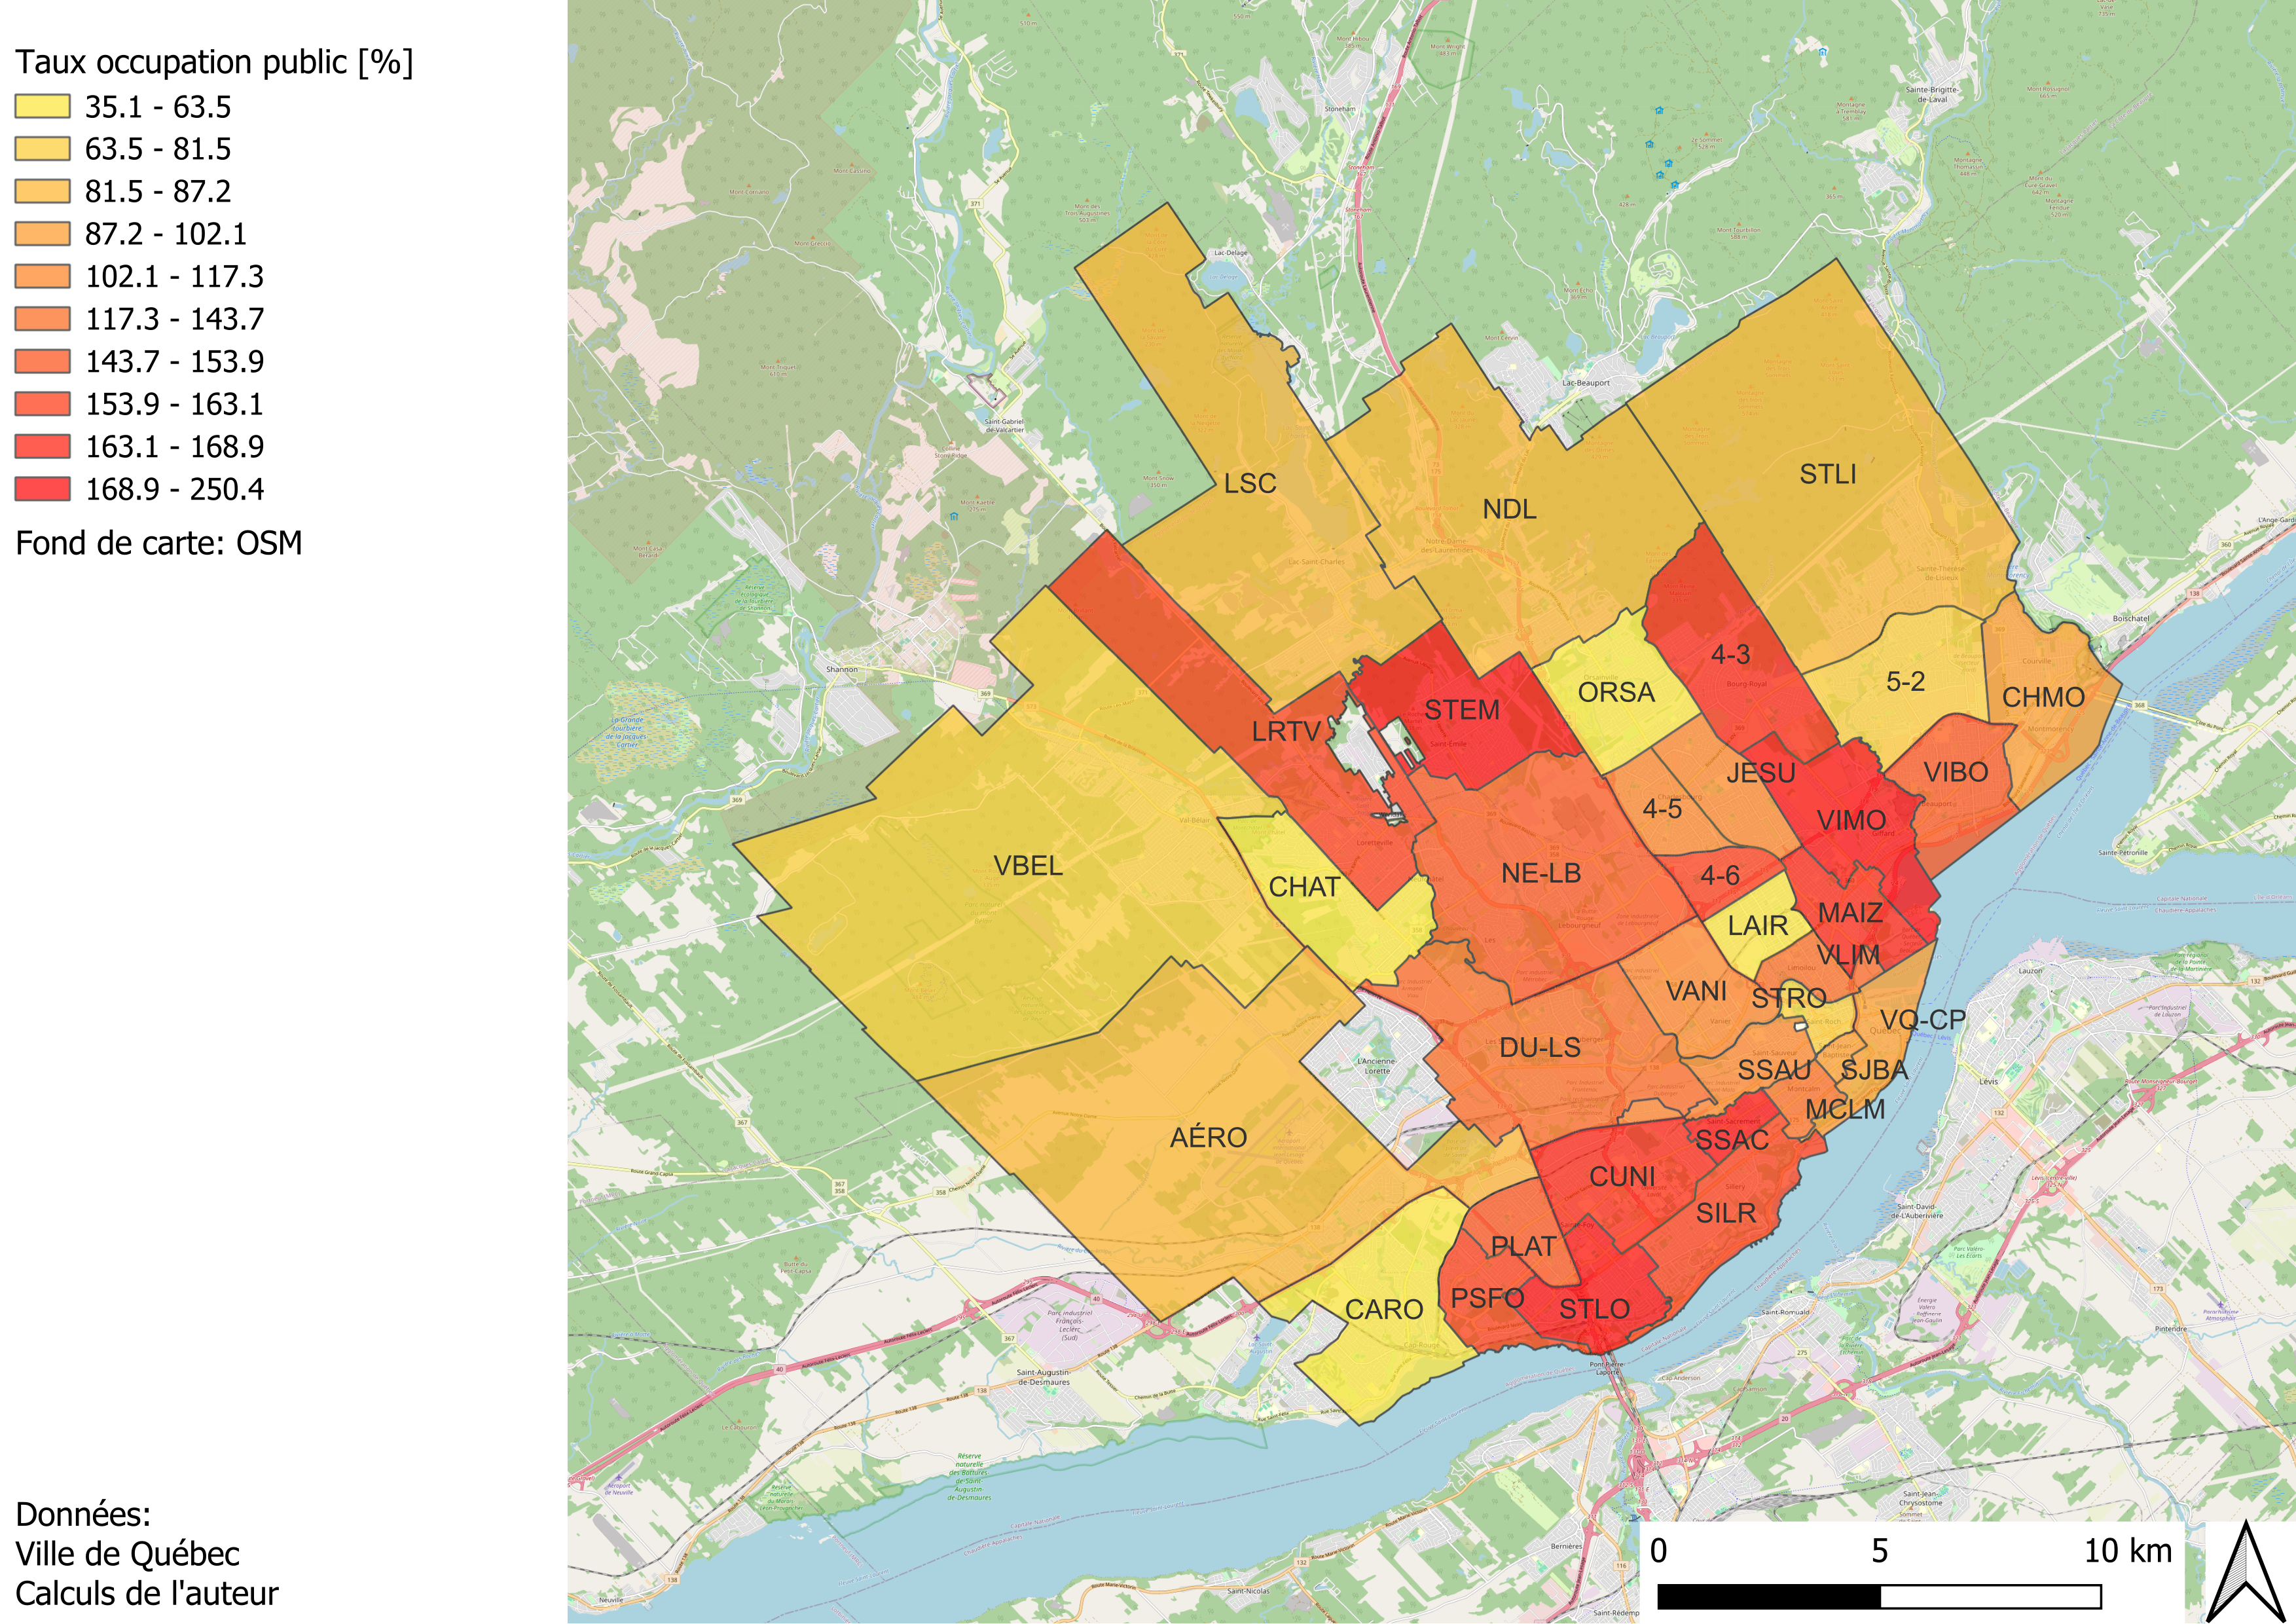
\includegraphics[width=0.8\linewidth]{images/taux-occup-public.png}
    \caption{Taux d'occupation public maximal prédit}
    \label{fig:occupancy-rate-public}
\end{figure}\clearpage
Finalement, la figure \ref{fig:occupancy-rate-residentiel} montre le taux d'occupation maximal résidentiel calculé de manière similaire.
\begin{figure}[H]
    \centering
    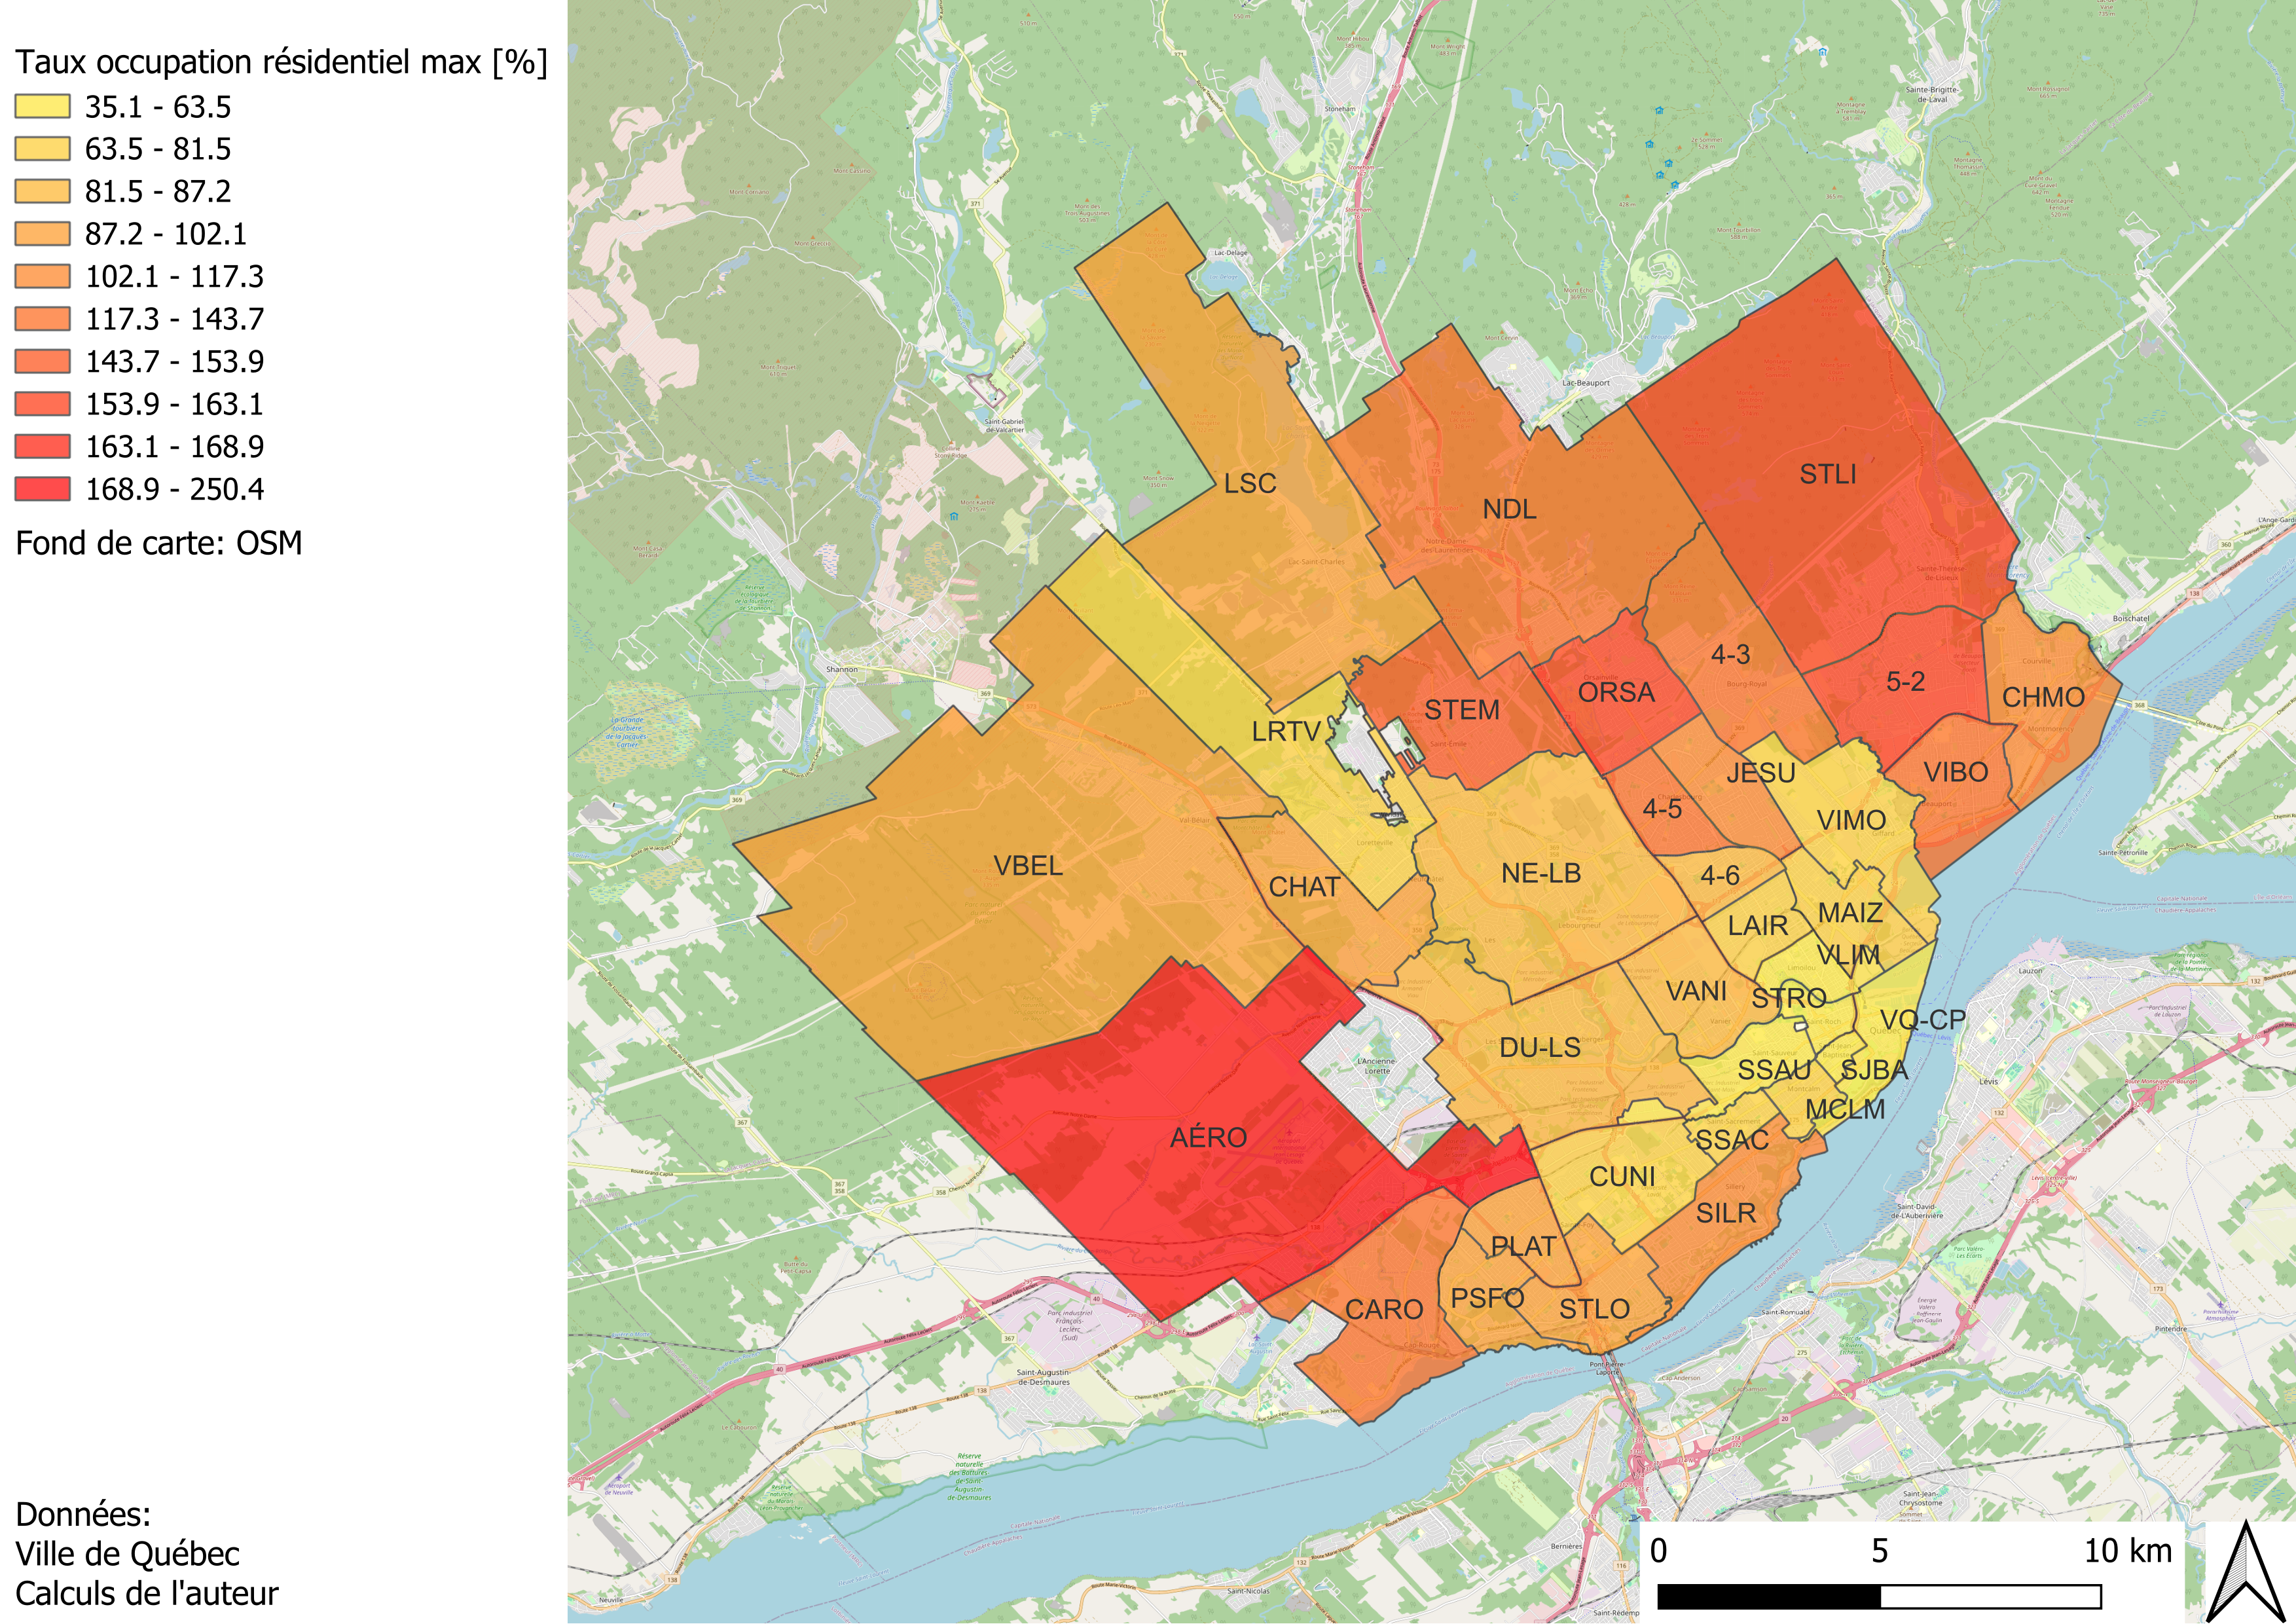
\includegraphics[width=0.8\linewidth]{images/taux-occup-res.png}
    \caption{Taux d'occupation résidentiel maximal prédit}
    \label{fig:occupancy-rate-residentiel}
\end{figure}

Ceci conclut la section sur les exemple d'analyse. Les données manquantes dans le rôle foncier et la complétion d'un processus de calibration des unités limite fortement la pertinence des constats, qui doivent tous être compris comme démonstratifs. La prochaine section donnera un récapitulatif du mémoire.